% This must be in the first 5 lines to tell arXiv to use pdfLaTeX, which is strongly recommended.
\pdfoutput=1
% In particular, the hyperref package requires pdfLaTeX in order to break URLs across lines.

\documentclass[11pt]{article}

% Change "review" to "final" to generate the final (sometimes called camera-ready) version.
% Change to "preprint" to generate a non-anonymous version with page numbers.
% \usepackage[review]{acl}
\usepackage{acl}

% Standard package includes
\usepackage{times}
\usepackage{latexsym}

% For proper rendering and hyphenation of words containing Latin characters (including in bib files)
\usepackage[T1]{fontenc}
% For Vietnamese characters
% \usepackage[T5]{fontenc}
% See https://www.latex-project.org/help/documentation/encguide.pdf for other character sets

% This assumes your files are encoded as UTF8
\usepackage[utf8]{inputenc}

% This is not strictly necessary, and may be commented out,
% but it will improve the layout of the manuscript,
% and will typically save some space.
\usepackage{microtype}

% This is also not strictly necessary, and may be commented out.
% However, it will improve the aesthetics of text in
% the typewriter font.
\usepackage{inconsolata}

%Including images in your LaTeX document requires adding
%additional package(s)
\usepackage{graphicx}

% If the title and author information does not fit in the area allocated, uncomment the following
%
%\setlength\titlebox{<dim>}
%
% and set <dim> to something 5cm or larger.
\usepackage{inconsolata}
\usepackage{graphicx}

\usepackage{enumitem}
\usepackage{multirow}
\usepackage{booktabs}
\usepackage{algorithm}
\usepackage{algorithmic}
\usepackage{tikz}
\usepackage{pgfplots}
\usepackage{graphicx}
\usepackage{subcaption}
\usepackage{pgf-pie}
\usepackage{enumitem}
\usepackage{pifont}
\usepackage{amsmath}
\usepackage{supertabular}
\usepackage{booktabs}
\numberwithin{equation}{section}
\usepackage{dsfont}
\usepgfplotslibrary{polar}


% \usepackage{inconsolata}
% \usepackage{ctex}
% \usepackage{algcompatible}
\pgfplotsset{compat=1.18}
\usepackage{bm}
\usepackage{xspace}
\usepackage{tcolorbox}
\usepackage{bbding}
\usepackage{wasysym}
\usepackage{amssymb}
\usepackage{fontawesome5}
\usepackage{arydshln}  
\usepackage{dashrule}


\newcommand{\ourmethod}{\textsc{Ours}\xspace}
\newcommand{\ourdataset}{\textsc{MultiTAT}\xspace}
\definecolor{cpurple}{rgb}{0.675, 0.573, 0.922}
\definecolor{cblue}{rgb}{0.310, 0.757, 0.910}
\definecolor{cgreen}{rgb}{0.310, 0.563, 0.214}
\definecolor{corange}{rgb}{1, 0.808, 0.329}
\definecolor{cred}{rgb}{0.8, 0.3, 0.3}
\definecolor{data_blue}{rgb}{0.809, 0.883, 0.949}
\definecolor{data_blue_light}{rgb}{0.930, 0.965, 1}
\definecolor{data_blue_dark}{rgb}{0.027, 0.215, 0.387}
\definecolor{annotator_pink}{rgb}{0.914, 0.816, 0.859}
\definecolor{gray}{rgb}{0.715, 0.715, 0.715}
\definecolor{gray_light}{rgb}{0.949, 0.949, 0.949}
% \definecolor{annotator_pink}{rgb}{0.297, 0.066, 0.188}
\definecolor{reasoner_green}{rgb}{0.848, 0.914, 0.824}
\newcommand{\datatext}[1]{{\color{data_blue_dark}#1}}
\newcommand{\textgray}[1]{{\color{gray}#1}}
\newcommand{\annotatortext}[1]{{\color{annotator_pink}#1}}
\newcommand{\greentext}[1]{{\color{reasoner_green}#1}}
% \newcommand{\textblue}[1]{{\color{softblue}#1}}
\providecommand{\longxu}[1]{{\protect\color{magenta}{[longxu: #1]}}}

\newtcolorbox{myexample}[2][]{
  colback=data_blue!40,
  colframe=data_blue,         % 设置边框颜色
  coltitle=black,
  title=\textbf{#2},
  fonttitle=\bfseries,
  #1,
}


% If the title and author information does not fit in the area allocated, uncomment the following
%
%\setlength\titlebox{<dim>}
%
% and set <dim> to something 5cm or larger.

\title{\ourdataset: Benchmarking Multilingual Table-and-Text\\Question Answering}
% MultiTAT: A Multilingual Benchmark for Question Answering on Table and Text
% MultiTAT: Benchmarking Multilingual Question Answering on Table and Text

% Author information can be set in various styles:
% For several authors from the same institution:
% \author{Author 1 \and ... \and Author n \\
%         Address line \\ ... \\ Address line}
% if the names do not fit well on one line use
%         Author 1 \\ {\bf Author 2} \\ ... \\ {\bf Author n} \\
% For authors from different institutions:
% \author{Author 1 \\ Address line \\  ... \\ Address line
%         \And  ... \And
%         Author n \\ Address line \\ ... \\ Address line}
% To start a seperate ``row'' of authors use \AND, as in
% \author{Author 1 \\ Address line \\  ... \\ Address line
%         \AND
%         Author 2 \\ Address line \\ ... \\ Address line \And
%         Author 3 \\ Address line \\ ... \\ Address line}
\author{
    Xuanliang Zhang\footnotemark[2], Dingzirui Wang\footnotemark[2], Keyan Xu, Qingfu Zhu, Wanxiang Che\\ 
    \texttt{\{xuanliangzhang, dzrwang, kyxu, qfzhu, car\}@ir.hit.edu.cn}\\
    Harbin Institute of Technology 
}

% \iffalse
% \author{First Author \\
%   Affiliation / Address line 1 \\
%   Affiliation / Address line 2 \\
%   Affiliation / Address line 3 \\
%   \texttt{email@domain} \\\And
%   Second Author \\
%   Affiliation / Address line 1 \\
%   Affiliation / Address line 2 \\
%   Affiliation / Address line 3 \\
%   \texttt{email@domain} \\}

\begin{document}
% \nolinenumbers
    \maketitle

\renewcommand{\thefootnote}{\fnsymbol{footnote}}
% \footnotetext[2]{The two authors contribute equally to this work.}
\footnotetext[2]{Equal contribution.}
% \footnotetext[1]{Corresponding author.}
\renewcommand{\thefootnote}{\arabic{footnote}}
    \begin{abstract}
    % TATQA是一个很重要的任务,旨在根据表格和文本的混合数据回答问题,广泛用于数据密集的领域
    Question answering on the hybrid context of tables and text (TATQA) is a critical task, with broad applications in data-intensive domains.
    % 然而,现在的TATQA数据集只局限于英语,存在以下缺点:
    % 1. 忽略了多语言TATQA的挑战,不能评测模型多语言TATQA的性能
    % 2. 和存在大量非英文的表格和文本的实际场景存在较大差距
    % However, existing TATQA datasets are limited to English, overlooking the challenges of multilingual TATQA, such as linguistic characteristics and variations in model performance across languages.
    However, existing TATQA datasets are limited to English, leading to several drawbacks:
    (i)~They overlook the challenges of multilingual TAT-QA and cannot assess model performance in the multilingual setting.
    (ii)~They do not reflect real-world scenarios where tables and texts frequently appear in non-English languages.
    % 所以,本文提出首个多语言TATQA数据集,来评测模型在多语言TATQA上的能力
    To address the limitations, we propose the first multilingual TATQA dataset (\ourdataset).
    % to evaluate TATQA capabilities in the multilingual setting.
    % 首先,我们从主流TATQA数据集中sample数据,并将其翻译为10种多样的语言
    Specifically, we sample data from $3$ mainstream TATQA datasets and translate it into $10$ diverse languages.
    % 为了提升模型在多语言TATQA任务上的性能,我们提出一个强baseline,能够提升模型处理不同语言的表格和文本中的信息的能力
    % To enhance performance on the multilingual TATQA task, we develop a baseline, \ourmethod, to align the model TATQA capabilities in English with other languages.
    To align the model TATQA capabilities in English with other languages, we develop a baseline, \ourmethod.
    % 实验结果表明,模型在我们数据集上的非英语相比英语上的性能平均下降18.9%,我们对此分析并总结了下降的原因
    Experimental results reveal that the performance on non-English data in \ourdataset drops by an average of $19.4\%$ compared to English, proving the necessity of \ourdataset.
    We further analyze the reasons for this performance gap.
    % 而我们的方法相比其他baseline平均提升2.6%,证明了我们方法的有效性
    Furthermore, \ourmethod outperforms other baselines by an average of $3.3$, demonstrating its effectiveness\footnote{Our data is available at \href{https://github.com/zhxlia/MULTITAT}{github.com/zhxlia/MULTITAT}}.


    % Question answering on the hybrid context of tables and text (TATQA) is a critical task, with broad applications in data-intensive domains. However, existing TATQA datasets are limited to English, leading to several drawbacks: (i) They overlook the challenges of multilingual TAT-QA and cannot assess model performance in the multilingual setting. (ii) They do not reflect real-world scenarios where tables and texts frequently appear in non-English languages. To address the limitations, we propose the first multilingual TATQA dataset (MULTITAT). Specifically, we sample data from 3 mainstream TATQA datasets and translate it into 10 diverse languages. To align the model TATQA capabilities in English with other languages, we develop a baseline, Ours. Experimental results reveal that the performance on non-English data in MULTITAT drops by an average of 19.4% compared to English, proving the necessity of MULTITAT. We further analyze the reasons for this performance gap. Furthermore, Ours outperforms other baselines by an average of 3.3, demonstrating its effectiveness.


    \end{abstract}


    \section{Introduction}
        

\section{Introduction}
\IEEEPARstart{I}{n} recent years, flourishing of Artificial Intelligence Generated Content (AIGC) has sparked significant advancements in modalities such as text, image, audio, and even video. 
Among these, AI-Generated Image (AGI) has garnered considerable interest from both researchers and the public.
Plenty of remarkable AGI models and online services, such as StableDiffusion\footnote{\url{https://stability.ai/}}, Midjourney\footnote{\url{https://www.midjourney.com/}}, and FLUX\footnote{\url{https://blackforestlabs.ai/}}, offer users an excellent creative experience.
However, users often remain critical of the quality of the AGI due to image distortions or mismatches with user intentions.
Consequently, methods for assessing the quality of AGI are becoming increasingly crucial to help improve the generative capabilities of these models.

Unlike Natural Scene Image (NSI) quality assessment, which focuses primarily on perception aspects such as sharpness, color, and brightness, AI-Generated Image Quality Assessment (AGIQA) encompasses additional aspects like correspondence and authenticity. 
Since AGI is generated on the basis of user text prompts, it may fail to capture key user intentions, resulting in misalignment with the prompt.
Furthermore, authenticity refers to how closely the generated image resembles real-world artworks, as AGI can sometimes exhibit logical inconsistencies.
While traditional IQA models may effectively evaluate perceptual quality, they are often less capable of adequately assessing aspects such as correspondence and authenticity.

\begin{figure}\label{fig:radar}
    \centering
    \includegraphics[width=1.0\linewidth]{figures/radar_plot.pdf}
    \caption{A comparison on quality, correspondence, and authenticity aspects of AIGCIQA2023~\cite{wang2023aigciqa2023} dataset illustrates the superior performance of our method.}
\end{figure}

Several methods have been proposed specifically for the AGIQA task, including metrics designed to evaluate the authenticity and diversity of generated images~\cite{gulrajani2017improved,heusel2017gans}. 
Nevertheless, these methods tend to compare and evaluate grouped images rather than single instances, which limits their utility for single image assessment.
Beginning with AGIQA-1k~\cite{zhang2023perceptual}, a series of AGIQA databases have been introduced, including AGIQA-3k~\cite{li2023agiqa}, AIGCIQA-20k~\cite{li2024aigiqa}, etc.
Concurrently, there has been a surge in research utilizing deep learning methods~\cite{zhou2024adaptive,peng2024aigc,yu2024sf}, which have significantly benefited from pre-trained models such as CLIP~\cite{radford2021learning}. 
These approaches enhance the analysis by leveraging the correlations between images and their descriptive texts.
While these models are effective in capturing general text-image alignments, they may not effectively detect subtle inconsistencies or mismatches between the generated image content and the detailed nuances of the textual description.
Moreover, as these models are pre-trained on large-scale datasets for broad tasks, they might not fully exploit the textual information pertinent to the specific context of AGIQA without task-specific fine-tuning.
To overcome these limitations, methods that leverage Multimodal Large Language Models (MLLMs)~\cite{wang2024large,wang2024understanding} have been proposed.
These methods aim to fully exploit the synergies of image captioning and textual analysis for AGIQA.
Although they benefit from advanced prompt understanding, instruction following, and generation capabilities, they often do not utilize MLLMs as encoders capable of producing a sequence of logits that integrate both image and text context.

In conclusion, the field of AI-Generated Image Quality Assessment (AGIQA) continues to face significant challenges: 
(1) Developing comprehensive methods to assess AGIs from multiple dimensions, including quality, correspondence, and authenticity; 
(2) Enhancing assessment techniques to more accurately reflect human perception and the nuanced intentions embedded within prompts; 
(3) Optimizing the use of Multimodal Large Language Models (MLLMs) to fully exploit their multimodal encoding capabilities.

To address these challenges, we propose a novel method M3-AGIQA (\textbf{M}ultimodal, \textbf{M}ulti-Round, \textbf{M}ulti-Aspect AI-Generated Image Quality Assessment) which leverages MLLMs as both image and text encoders. 
This approach incorporates an additional network to align human perception and intentions, aiming to enhance assessment accuracy. 
Specially, we distill the rich image captioning capability from online MLLMs into a local MLLM through Low-Rank Adaption (LoRA) fine-tuning, and train this model with human-labeled data. The key contributions of this paper are as follows:
\begin{itemize}
    \item We propose a novel AGIQA method that distills multi-aspect image captioning capabilities to enable comprehensive evaluation. Specifically, we use an online MLLM service to generate aspect-specific image descriptions and fine-tune a local MLLM with these descriptions in a structured two-round conversational format.
    \item We investigate the encoding potential of MLLMs to better align with human perceptual judgments and intentions, uncovering previously underestimated capabilities of MLLMs in the AGIQA domain. To leverage sequential information, we append an xLSTM feature extractor and a regression head to the encoding output.
    \item Extensive experiments across multiple datasets demonstrate that our method achieves superior performance, setting a new state-of-the-art (SOTA) benchmark in AGIQA.
\end{itemize}

In this work, we present related works in Sec.~\ref{sec:related}, followed by the details of our M3-AGIQA method in Sec.~\ref{sec:method}. Sec.~\ref{sec:exp} outlines our experimental design and presents the results. Sec.~\ref{sec:limit},~\ref{sec:ethics} and~\ref{sec:conclusion} discuss the limitations, ethical concerns, future directions and conclusions of our study.
    
    \section{\ourdataset}
        \label{sec:dataset}
        % 我们数据集的输入为表格、文本和相关的问题,输出为问题的回答
The input of \ourdataset consists of a question, the hybrid context including the table and text, and the output is the answer to the question. 
% 并且,我们为每个问题标注了rationale
Additionally, we annotate the rationale, which is the reasoning process of answering the question in \ourdataset. 
% 我们称每个问题,以及它对应的表格、文本、rationale和答案为一个instance
We refer to each question, along with its corresponding table, text, rationale, and answer, as an instance. 
% 我们为每个instance标注了10种非英语的多样的语言
For each instance, we annotate $11$ diverse languages.
% 首先,我们介绍我们数据集的构建过程,采用了自动翻译和人工纠错相结合的方式,following前人工作,如图所示
We first describe the construction process of \ourdataset, which combines automatic generation with manual error correction, following previous works \cite{peng-etal-2024-humanevalxl,singh-etal-2024-indicgenbench,MultiSpider}, as shown in Figure~\ref{fig:framework}.

\begin{figure*}
    \centering
    \includegraphics[width=.85\linewidth]{fig/framework.pdf}
    % \vspace{-0.5em}
    \caption{
    % 我们数据集构建的流程
    The process of constructing \ourdataset.
    % 蓝色框代表数据,白色实线框代表构造步骤
    The \colorbox{data_blue_light}{\datatext{blue}} boxes represent the data, and the white solid boxes represent the construction steps.
    }
    \label{fig:framework}
\end{figure*}

\begin{table*}[t]
    \centering
    \small
    \begin{tabular}{@{}l l l l c c c c@{}}
\toprule
\multirow{2}{*}{\textbf{Dataset}} & \multirow{2}{*}{\textbf{Domain}} & \multirow{2}{*}{\textbf{Scale}} & \multirow{2}{*}{\textbf{Answer Type}} & \multicolumn{3}{c}{\textbf{Answer Source}} & \multirow{2}{*}{\textbf{Total}}\\ 
\cmidrule(lr){5-7}
 & & & & \textbf{Text} & \textbf{Table} & \textbf{Hybrid} \\
\midrule
HybridQA~\cite{chen-etal-2020-hybridqa} & Wikipedia & $50$ & Span & $0$ & $0$ & $50$ & $50$ \\
\midrule
\multirow{3}{*}{TAT-QA~\cite{zhu-etal-2021-tat}} & \multirow{3}{*}{Finance} & \multirow{3}{*}{$100$} & Span & $10$ & $10$ & $20$ & $40$ \\ 
 & & & Arithmetic & $10$ & $10$ & $30$ & $50$ \\ 
 & & & Count & $2$ & $3$ & $5$ & $10$ \\
\midrule
\multirow{2}{*}{SciTAT~\cite{zhang2024scitat}} & \multirow{2}{*}{Science} & \multirow{2}{*}{$100$} & Span & $10$ & $20$ & $20$ & $50$ \\
 & & & Arithmetic & $10$ & $20$ & $20$ & $50$ \\
\midrule
Total & - & $250$ & - & $42$ & $63$ & $145$ & $250$ \\
\bottomrule
\end{tabular}
    % \vspace{-0.5em}
    \caption{
    % 我们数据集中数据的分布
    The distribution of English data, including answer types and answer sources in \ourdataset, sourced from three mainstream datasets.
    % 表中列出的是每个数据集拥有的所有答案类型
    The listed answer types are the all answer types corresponding to each dataset.
    }
    \label{tab:answer_statistics}
\end{table*}


\subsection{Data Preparation}
We first collect English data from existing datasets and select languages to translate them.

\subsubsection{Source Data Collection}
% 我们分别选取了wikipedia,金融和科学领域的HybridQA, TAT-QA和SciTAT数据集作为我们的数据来源,因为这三个领域是目前TATQA任务主要分布的领域
We select HybridQA~\cite{chen-etal-2020-hybridqa}, TAT-QA~\cite{zhu-etal-2021-tat}, and SciTAT~\cite{zhang2024scitat} datasets from the Wikipedia, finance, and science domains as our data sources, as these three domains are the primary areas where TATQA tasks are currently distributed (see Table~\ref{tab:comparison_tat}). 
% 为了令我们的数据集在不同的答案来源和答案类型上均匀分布,我们按照表格中的比例从三个数据集共采样了250条数据,如表所示
To ensure an even distribution of different answer types and answer sources in \ourdataset, we sample a total of $250$ instances from the three datasets according to the proportions shown in Table~\ref{tab:answer_statistics}. 
% 其中,HybridQA数据集只采样了50条是由于其答案来源和类型较为单一
Among them, only $50$ instances are sampled from HybridQA due to its relatively limited answer sources and types. 

\subsubsection{Target Language Selection}
% 我们选取了除英语之外的10种语言覆盖8个语系,分别是Bengali (BN), Chinese (ZH), French (FR), German (DE), Japanese (JA), Russian (RU), Spanish (ES), Swahili (SW), Telugu (TE), and Thai (TH),follow前人工作.
For \ourdataset, we select $11$ languages, covering $8$ language families: Bengali (bn), Chinese (zh), English (en), French (fr), German (de), Japanese (ja), Russian (ru), Spanish (es), Swahili (sw), Telugu (te), and Thai (th), following the previous benchmark \cite{shi2023MGSM}. 
% 并且,我们在所有语言中都保持了原数据集中答案的阿拉伯数字,以便评测(引)
Additionally, we preserve the Arabic numerals from the original datasets across all languages to facilitate evaluation \cite{shi2023MGSM}.

\subsection{Rationale Annotation}
\label{subsec:Rationale Annotation}
% \paragraph{Rationale Generation}
% 在本节,我们首先展示了如何使用LLM结合人工修改来标注rationale
We first demonstrate how to annotate English rationales by employing the large language model (LLM) in combination with manual refinement. 
% 我们首先使用gpt-4o完成英文rationale的标注,因为其强大的推理能力以及instruction-following的能力
We use \texttt{gpt-4o}~\cite{openai2024gpt4technicalreport} to complete \textbf{rationale generation} due to its strong reasoning and instruction-following capabilities. 
% 具体地,我们将问题,相关的表格和文本以及答案输入LLM,提示模型生成推理过程。
Specifically, we input the question, relevant tables and texts, and the answer into the LLM, prompting the LLM to generate the corresponding rationale.
% \paragraph{Human Refinement}
% 由于LLM不能保证推理的正确性,我们采用人工校验及修改
Since LLMs cannot guarantee the accuracy of reasoning, we employ \textbf{manual refinement}. 
% 对于模型生成的推理过程,我们提示标注者判断英语rationale的正确性,对于错误的进行修改
The annotators are instructed to evaluate the accuracy of the generated rationale and make corrections where necessary.

\subsection{Instance Translation}
\label{subsec:Instance Translation}
% 在本节,我们介绍使用LLM结合人工标注将英文instance翻译为10种语言
In this section, we describe the process of combining the LLM with human annotations to translate English instances into $10$ languages. 
% \paragraph{Machine Translation}
% 我们选择gpt-4o,因为其强大的翻译能力
For \textbf{machine translation}, we select \texttt{gpt-4o} because of its strong translation capabilities \cite{yan2024gpt4vshumantranslators,hu-etal-2024-gentranslate}. 
% 我们将instance输入LLM,分别提示模型翻译为10种目标语言
Specifically, we input each instance into the LLM, with prompts to translate it into the target languages, respectively. 
% \paragraph{Human Refinement}
% 为了评测翻译的正确性,我们follow前人工作使用gpt-4o将翻译成目标语言的instance翻译回英语,计算其和原本英语版本的F1
To assess the accuracy of the translations, we use \texttt{gpt-4o} to translate the target language instances back into English, and calculate the F1 score between the back-translated version and the original English instance following previous works \cite{peng-etal-2024-humanevalxl}. 
% 对于F1<0.6的instance,我们提示标注者使用谷歌翻译重新翻译并检查,直至回译和原始英文版本一致
For instances with an F1 score below $0.6$, we prompt annotators to complete \textbf{manual refinement} by using Google Translation for a new translation.
% and verification, iterating until the back-translated instances align with the original English version.

% \subsection{Initial Annotation}
% % 我们首先使用LLM完成英文rationale的标注,以及将英文instance翻译为10种语言
% We first employ large language models (LLMs) to annotate the English rationales and translate the English instances into ten languages. 
% % 具体地,我们使用的是gpt-4o,因为其强大的推理能力,instruction-following的能力,以及翻译能力
% Specifically, we use \texttt{gpt-4o}~\cite{openai2024gpt4technicalreport}, given its strong reasoning ability, proficiency in instruction-following, and translation capabilities.
% % 1. 对于rationale的标注,我们将问题,相关的表格和文本以及答案输入LLM,提示模型生成推理过程。
% (\emph{i})~For rationale annotation, we input the question, relevant tables and text, and the answer into the LLM, prompting the model to generate the reasoning process. 
% % 在经过人工校验及修改后(过程见S2.3),我们将每个instance翻译为目标语言。
% After manual verification and modification (as described in Section \S\ref{subsec:Human Annotation}), we translate each instance into the target languages.
% % 2. 对于instance的翻译,我们将表格,文本,问题,rationale和答案都输入LLM,分别提示模型翻译为10种目标语言
% (\emph{ii})~For instance translation, we input the tables, text, question, rationale, and answer into the LLM, prompting the model to translate them into the target languages, respectively.
% % 我们标注过程中使用的prompt在附录中提供
% % The prompts used during the annotation process are provided in Appendix.

% \subsection{Human Refinement}
% \label{subsec:Human Refinement}
% % 由于LLM不能保证推理以及翻译的正确性,我们采用人工校验及修改
% Since LLMs cannot guarantee the accuracy of reasoning and translation, we employ manual verification and correction. 
% % 对于推理过程,我们提示标注者判断英语rationale的正确性,对于错误的进行修改
% (\emph{i})~For the rationale, we instruct the annotators to assess the correctness of the English rationale, making corrections where necessary. 
% % 对于翻译过程,我们follow前人工作采用回译进行判断。
% (\emph{ii})~For the translation, we follow previous works by using back-translation for validation \cite{peng-etal-2024-humanevalxl}. 
% % 具体来说,我们使用gpt-4o将翻译成目标语言的instance翻译回英语,计算其和原本英语版本的F1
% Specifically, we utilize \texttt{gpt-4o} to translate target language instances back into English and compute the F1 score between the back-translated version and the original English version. 
% % 对于F1<0.6的instance,我们提示标注者使用谷歌翻译重新翻译并检查,直至回译和原始英文版本一致
% For instances with an F1 score below $0.6$, we instruct the annotators to use Google Translation for a new translation and review it until the back-translated version matches the original English text.

\subsection{Quality Control}
% 为了保证我们的数据集中数据的质量,我们采取了严格的质量控制策略
To ensure the quality of \ourdataset, we implement rigorous quality control strategies.
% 首先,回译是广泛被前人采用的评价翻译质量的方法。
% First, back-translation is a widely adopted method for evaluating translation quality. 
% 并且,我们的方法是结合人工校验的gpt-4o和谷歌翻译的融合学习的结果,有着优越的翻译性能
% Our translation process, which combines the results of human-validated \texttt{gpt-4o} and Google Translation through ensemble learning, demonstrates superior translation performance. 
% \paragraph{Competent Annotators}
% 我们雇佣的标注者均为研究生及以上学历,精通英语,并支付给他们每条数据$1的费用
The annotators we hire hold graduate-level degrees, are proficient in English and are compensated with $\$1$ per data instance. 
% 我们首先对标注者进行培训,使其了解标注的要求以及标注工具的使用(见附录)
We first train the annotators to familiarize them with the annotation requirements and the use of the annotation tool (see Appendix~\ref{subsec:Annotator Training Process}). 
% 然后,我们令其试标注20条数据,检查他们标注的结果并给出反馈以及修改意见
Then, they try to annotate $20$ instances, and we review their annotations, providing feedback and suggestions for revisions.

% \paragraph{Quality Inspection}
% 为了进一步确保翻译的质量,我们选择了低资源语言,包括孟加拉语、斯瓦希里语以及泰卢固语,对我们的数据集的翻译进行评测
% To further ensure the quality of the translations, we select low-resource languages, including Bengali, Swahili, and Telugu, to evaluate the translations in \ourdataset. 
% % 具体来说,我们分别请了母语为这三种语言且精通英语的标注者分别对这些语言在我们数据集中的问题,对照英文的原始问题对翻译的流畅性、充分性和一致性进行打分
% Specifically, native speakers of these languages, who are also proficient in English, are asked to rate the fluency, adequacy, and consistency of the translated questions by comparing them to the original English questions in \ourdataset. 
% % 最终平均得分分别为,证明了我们数据集翻译的质量
% The final average scores is , demonstrating the high quality of \ourdataset. 
% % 我们将具体分值放在了附录
% Detailed annotation process and scoring information are provided in Appendix.

% \begin{table}[t]
%     \centering
%     \small
%     \begin{tabular}{@{}lc@{}}
\toprule
%  & \# \\ 
% \midrule
Question       & $250$   \\
Hybrid Contexts & $233$   \\
Avg. Rows      & $10.2$  \\
Avg. Columns   & $4.7$   \\
Avg. Paragraphs & $5.3$   \\
\bottomrule
\end{tabular}
%     \vspace{-0.5em}
%     \caption{
%     % 我们数据集中数据的分布
%     The basic statistics of \ourdataset.
%     }
%     \label{tab:basic_statistics}
% \end{table}

\subsection{Data Analysis}
% 我们展示了我们数据集的基本数据的统计结果,如表1和表2所示
We show the data distribution of \ourdataset in Table~\ref{tab:answer_statistics}.
% 我们数据集中的250个问题涉及233个混合上下文,其中每个混合上下文包括1个表格和平均5.3个段落。其中每个表格平均有10.2行和4.7列
The $250$ questions in \ourdataset involve $233$ hybrid contexts, each of which includes $1$ table and an average of $5.3$ paragraphs. 
Each table has an average of $10.2$ rows and $4.7$ columns.

\begin{figure*}[t]
    \centering
    \includegraphics[width=.95\linewidth]{fig/method.pdf}
    % \vspace{-0.5em}
    \caption{
    % 我们方法的示意图,我们方法分为两步:
    The overview of \ourmethod, which includes two modules:
    % 1. Linking根据问题链接到表格或文本中相关的信息
    (\emph{i})~\textbf{Linking}: Mapping the entities in the question to the relevant information in tables or text, which are marked with \datatext{\textbf{blue}} in the left part.
    % 2. Reasoning根据相关信息生成代码求解
    (\emph{ii})~\textbf{Reasoning}: Generating programs to solve the question using the information.
    % 例子和图一中的例子一致
    % The example is consistent with the Chinese one shown in Figure~\ref{fig:intro}.
    % 我们以中文TATQA的输入为例,括号中的灰色文字为对应的英文
    We take the Chinese TATQA input as an example, with the corresponding English text provided in \colorbox{gray_light}{\textgray{(gray)}}.
    % within parentheses.
    }
    \label{fig:method}
\end{figure*}


    
    \section{\ourmethod}
        \label{sec:methodology}
        \section{Methodology}

\method consists of three key components.
(1) A hierarchical linguistic structure with supporting corpora for linguistic mechanism analysis;
(2) Linguistic feature analysis for interpreting SAE extracted features; and
(3) Linguistic feature intervention for causal analysis and LLM steering.


\begin{figure*}[tp]
    \centering
    \includegraphics[width=0.97\textwidth]{figure/methology.pdf}
    \vspace{-0.01in}
    \caption{
    The overall framework of \method.
    We propose a large-model linguistic mechanism framework encompassing six dimensions and select classical features from these dimensions for experimentation. 
    The experimental workflow is as follows: 
    (1) Construct minimal contrast and counterfactual datasets; 
    (2) Extract features and evaluate their relevance by analyzing the activation values of base vectors on the datasets; 
    (3) Intervene in the model output by modifying activation values and assess causality using an LLM as a judge.
    }\label{fig:method}
\end{figure*}


\subsection{Linguistic Structure}

\paragraph{Hierarchical Linguistic Structure.}
To systematically interpret the language capabilities of large models, we adopt a six level structure based on theoretical linguistics~\cite{fromkin2017introduction}: phonetics, phonology, morphology, syntax, semantics, and pragmatics.
The structure follows a logical progression from the external, physical realization of sound to the internal, contextual understanding of meaning. 
Each linguistic capability contains several concrete linguistic features, \textit{e.g.,} semantics level includes metaphor, simile, \textit{etc}.
We provide the exact definition for each linguistic capability in Appendix~\ref{app:ling}

% Our structure provides a comprehensive and modular way to explain how large language models achieve different levels of language ability. 
% By finding linguistic features at different levels in the SAE latent space of large models, we can more accurately reveal how these models represent and process natural language, thereby revealing the underlying mechanism of the models' language ability.
% This mechanism can also bring linguists a clearer understanding of how language knowledge is organized.

\paragraph{Dataset Construction.}
The sparse feature activation distribution of SAE is closely related to the conditions under which their corresponding linguistic features hold in linguistic knowledge.
To find the linguistic features and evaluate its dominance, we propose a method to construct the dataset and analyze feature activation frequencies.

For each linguistic feature, we first construct a set of sentences that significantly align with the desired feature. 
The feature activation representing this linguistic feature in SAE’s hidden space will be significantly activated on these sentences. 
However, this is not enough to accurately identify them, as there are some background noise vectors that are activated on all sentences in the dataset and interfere with our judgment. 
We need to include a control group without the feature in the constructed sentences. 

We introduce two types of control groups: minimal pairs and counterfactual sentences. Minimal pairs are constructed by changing only the part of a sentence that corresponds to a particular linguistic feature, while keeping all other parts unchanged. However, this approach often results in syntactically incorrect sentences.

To overcome this limitation, we also construct fully grammatically correct control groups, called counterfactual sentences, which differ from the original sentence only in terms of its linguistic features. Detailed dataset construction procedures are provided in Appendix~\ref{app:data_construction}.

\subsection{Feature Analysis}
We propose a causal probability approach to evaluate the relationship between extracted linguistic features and their activation on sentences containing those features. 

For a given feature \(x\), we define two key probabilities. The \emph{Probability of Necessity} (PN) quantifies how necessary the feature is for the activation of a corresponding base vector, while the \emph{Probability of Sufficiency} (PS) measures the likelihood that introducing the feature triggers activation. These probabilities are then combined into a \emph{Feature Representation Confidence} (FRC) score, which assesses both the representational capacity of the SAE latent space and the discriminative ability of the feature to identify the corresponding linguistic phenomenon. 

During feature analysis, we calculate the FRS on both the minimal contrast dataset and the counterfactual dataset, then average the results. This average more accurately reflects the ability of the base vectors to represent the linguistic features. Detailed definitions and calculation methods are provided in Appendix~\ref{app:frc}.



\subsection{Feature Intervention}
When we modify the values of SAE’s activation during forward propagation, we expect that such targeted interventions will influence the model’s behavior. 
However, our experiments show that altering only a small subset of features may not significantly impact the output—likely because linguistic phenomena are represented by multiple features across various layers. 
To assess the true impact of these interventions, we use a large language model as a judge. For each linguistic feature, we conduct both ablation and enhancement experiments. 
In the ablation experiment, we set the target feature’s activation to $0$, and in the enhancement experiment, we set it to $10$. 
In both cases, we also perform baseline experiments by randomly selecting 25 base vectors from the same layer.

For brevity, we denote the interventions as follows: let \(I_{abl}^{T}\) denote the targeted ablation intervention, \(I_{abl}^{B}\) the baseline ablation intervention, \(I_{enh}^{T}\) the targeted enhancement intervention, and \(I_{enh}^{B}\) the baseline enhancement intervention.

Let \(P_{abl}^{T}\) and \(P_{abl}^{B}\) denote the success probabilities (\textit{i.e.,} the probability that the intended change in the linguistic phenomenon is observed) for the targeted and baseline ablation experiments. The normalized ablation effect is then defined as
\[
\begin{aligned}
E_{abl} &= P_{abl}^{T} - P_{abl}^{B} \\
        &= \frac{P(Y=0 \mid I_{abl}^{T}) - P(Y=0 \mid I_{abl}^{B})}{P(Y=0 \mid I_{abl}^{T})}.
\end{aligned}
\]
Similarly, let \(P_{enh}^{T}\) and \(P_{enh}^{B}\) be the success probabilities for the targeted and baseline enhancement experiments, with \(Y=1\) indicating the presence of the phenomenon. The normalized enhancement effect is given by
\[
\begin{aligned}
E_{enh} &= P_{enh}^{T} - P_{enh}^{B} \\
        &= \frac{P(Y=1 \mid I_{enh}^{T}) - P(Y=1 \mid I_{enh}^{B})}{1 - P(Y=1 \mid I_{enh}^{B})}.
\end{aligned}
\]

Finally, we define the Feature Intervention Confidence (FIC) score as the harmonic mean of the normalized ablation and enhancement effects:
\[
\text{FIC} = \frac{2\, E_{abl}\, E_{enh}}{E_{abl} + E_{enh}}.
\]
When calculating FIC, if one or both of the $E$ values are negative, we incorporate a penalty coefficient $w$ to reflect the weakened or lost causality in such cases. 
This FIC score provides a balanced measure of how effectively targeted interventions, as opposed to random ones, influence the model’s output with respect to specific linguistic features.
The details for FIC are shown in Appendix~\ref{app:fic}.
% The detailed computation can be found in Appendix~\ref{app:fic}.
    
    \section{Experiments}
        \label{sec:experiments}
        \subsection{Settings}

\begin{table*}[ht]
\centering
\tiny
% This must be in the first 5 lines to tell arXiv to use pdfLaTeX, which is strongly recommended.
\pdfoutput=1
% In particular, the hyperref package requires pdfLaTeX in order to break URLs across lines.

\documentclass[11pt]{article}

% Change "review" to "final" to generate the final (sometimes called camera-ready) version.
% Change to "preprint" to generate a non-anonymous version with page numbers.
\usepackage{acl}

% Standard package includes
\usepackage{times}
\usepackage{latexsym}

% Draw tables
\usepackage{booktabs}
\usepackage{multirow}
\usepackage{xcolor}
\usepackage{colortbl}
\usepackage{array} 
\usepackage{amsmath}

\newcolumntype{C}{>{\centering\arraybackslash}p{0.07\textwidth}}
% For proper rendering and hyphenation of words containing Latin characters (including in bib files)
\usepackage[T1]{fontenc}
% For Vietnamese characters
% \usepackage[T5]{fontenc}
% See https://www.latex-project.org/help/documentation/encguide.pdf for other character sets
% This assumes your files are encoded as UTF8
\usepackage[utf8]{inputenc}

% This is not strictly necessary, and may be commented out,
% but it will improve the layout of the manuscript,
% and will typically save some space.
\usepackage{microtype}
\DeclareMathOperator*{\argmax}{arg\,max}
% This is also not strictly necessary, and may be commented out.
% However, it will improve the aesthetics of text in
% the typewriter font.
\usepackage{inconsolata}

%Including images in your LaTeX document requires adding
%additional package(s)
\usepackage{graphicx}
% If the title and author information does not fit in the area allocated, uncomment the following
%
%\setlength\titlebox{<dim>}
%
% and set <dim> to something 5cm or larger.

\title{Wi-Chat: Large Language Model Powered Wi-Fi Sensing}

% Author information can be set in various styles:
% For several authors from the same institution:
% \author{Author 1 \and ... \and Author n \\
%         Address line \\ ... \\ Address line}
% if the names do not fit well on one line use
%         Author 1 \\ {\bf Author 2} \\ ... \\ {\bf Author n} \\
% For authors from different institutions:
% \author{Author 1 \\ Address line \\  ... \\ Address line
%         \And  ... \And
%         Author n \\ Address line \\ ... \\ Address line}
% To start a separate ``row'' of authors use \AND, as in
% \author{Author 1 \\ Address line \\  ... \\ Address line
%         \AND
%         Author 2 \\ Address line \\ ... \\ Address line \And
%         Author 3 \\ Address line \\ ... \\ Address line}

% \author{First Author \\
%   Affiliation / Address line 1 \\
%   Affiliation / Address line 2 \\
%   Affiliation / Address line 3 \\
%   \texttt{email@domain} \\\And
%   Second Author \\
%   Affiliation / Address line 1 \\
%   Affiliation / Address line 2 \\
%   Affiliation / Address line 3 \\
%   \texttt{email@domain} \\}
% \author{Haohan Yuan \qquad Haopeng Zhang\thanks{corresponding author} \\ 
%   ALOHA Lab, University of Hawaii at Manoa \\
%   % Affiliation / Address line 2 \\
%   % Affiliation / Address line 3 \\
%   \texttt{\{haohany,haopengz\}@hawaii.edu}}
  
\author{
{Haopeng Zhang$\dag$\thanks{These authors contributed equally to this work.}, Yili Ren$\ddagger$\footnotemark[1], Haohan Yuan$\dag$, Jingzhe Zhang$\ddagger$, Yitong Shen$\ddagger$} \\
ALOHA Lab, University of Hawaii at Manoa$\dag$, University of South Florida$\ddagger$ \\
\{haopengz, haohany\}@hawaii.edu\\
\{yiliren, jingzhe, shen202\}@usf.edu\\}



  
%\author{
%  \textbf{First Author\textsuperscript{1}},
%  \textbf{Second Author\textsuperscript{1,2}},
%  \textbf{Third T. Author\textsuperscript{1}},
%  \textbf{Fourth Author\textsuperscript{1}},
%\\
%  \textbf{Fifth Author\textsuperscript{1,2}},
%  \textbf{Sixth Author\textsuperscript{1}},
%  \textbf{Seventh Author\textsuperscript{1}},
%  \textbf{Eighth Author \textsuperscript{1,2,3,4}},
%\\
%  \textbf{Ninth Author\textsuperscript{1}},
%  \textbf{Tenth Author\textsuperscript{1}},
%  \textbf{Eleventh E. Author\textsuperscript{1,2,3,4,5}},
%  \textbf{Twelfth Author\textsuperscript{1}},
%\\
%  \textbf{Thirteenth Author\textsuperscript{3}},
%  \textbf{Fourteenth F. Author\textsuperscript{2,4}},
%  \textbf{Fifteenth Author\textsuperscript{1}},
%  \textbf{Sixteenth Author\textsuperscript{1}},
%\\
%  \textbf{Seventeenth S. Author\textsuperscript{4,5}},
%  \textbf{Eighteenth Author\textsuperscript{3,4}},
%  \textbf{Nineteenth N. Author\textsuperscript{2,5}},
%  \textbf{Twentieth Author\textsuperscript{1}}
%\\
%\\
%  \textsuperscript{1}Affiliation 1,
%  \textsuperscript{2}Affiliation 2,
%  \textsuperscript{3}Affiliation 3,
%  \textsuperscript{4}Affiliation 4,
%  \textsuperscript{5}Affiliation 5
%\\
%  \small{
%    \textbf{Correspondence:} \href{mailto:email@domain}{email@domain}
%  }
%}

\begin{document}
\maketitle
\begin{abstract}
Recent advancements in Large Language Models (LLMs) have demonstrated remarkable capabilities across diverse tasks. However, their potential to integrate physical model knowledge for real-world signal interpretation remains largely unexplored. In this work, we introduce Wi-Chat, the first LLM-powered Wi-Fi-based human activity recognition system. We demonstrate that LLMs can process raw Wi-Fi signals and infer human activities by incorporating Wi-Fi sensing principles into prompts. Our approach leverages physical model insights to guide LLMs in interpreting Channel State Information (CSI) data without traditional signal processing techniques. Through experiments on real-world Wi-Fi datasets, we show that LLMs exhibit strong reasoning capabilities, achieving zero-shot activity recognition. These findings highlight a new paradigm for Wi-Fi sensing, expanding LLM applications beyond conventional language tasks and enhancing the accessibility of wireless sensing for real-world deployments.
\end{abstract}

\section{Introduction}

In today’s rapidly evolving digital landscape, the transformative power of web technologies has redefined not only how services are delivered but also how complex tasks are approached. Web-based systems have become increasingly prevalent in risk control across various domains. This widespread adoption is due their accessibility, scalability, and ability to remotely connect various types of users. For example, these systems are used for process safety management in industry~\cite{kannan2016web}, safety risk early warning in urban construction~\cite{ding2013development}, and safe monitoring of infrastructural systems~\cite{repetto2018web}. Within these web-based risk management systems, the source search problem presents a huge challenge. Source search refers to the task of identifying the origin of a risky event, such as a gas leak and the emission point of toxic substances. This source search capability is crucial for effective risk management and decision-making.

Traditional approaches to implementing source search capabilities into the web systems often rely on solely algorithmic solutions~\cite{ristic2016study}. These methods, while relatively straightforward to implement, often struggle to achieve acceptable performances due to algorithmic local optima and complex unknown environments~\cite{zhao2020searching}. More recently, web crowdsourcing has emerged as a promising alternative for tackling the source search problem by incorporating human efforts in these web systems on-the-fly~\cite{zhao2024user}. This approach outsources the task of addressing issues encountered during the source search process to human workers, leveraging their capabilities to enhance system performance.

These solutions often employ a human-AI collaborative way~\cite{zhao2023leveraging} where algorithms handle exploration-exploitation and report the encountered problems while human workers resolve complex decision-making bottlenecks to help the algorithms getting rid of local deadlocks~\cite{zhao2022crowd}. Although effective, this paradigm suffers from two inherent limitations: increased operational costs from continuous human intervention, and slow response times of human workers due to sequential decision-making. These challenges motivate our investigation into developing autonomous systems that preserve human-like reasoning capabilities while reducing dependency on massive crowdsourced labor.

Furthermore, recent advancements in large language models (LLMs)~\cite{chang2024survey} and multi-modal LLMs (MLLMs)~\cite{huang2023chatgpt} have unveiled promising avenues for addressing these challenges. One clear opportunity involves the seamless integration of visual understanding and linguistic reasoning for robust decision-making in search tasks. However, whether large models-assisted source search is really effective and efficient for improving the current source search algorithms~\cite{ji2022source} remains unknown. \textit{To address the research gap, we are particularly interested in answering the following two research questions in this work:}

\textbf{\textit{RQ1: }}How can source search capabilities be integrated into web-based systems to support decision-making in time-sensitive risk management scenarios? 
% \sq{I mention ``time-sensitive'' here because I feel like we shall say something about the response time -- LLM has to be faster than humans}

\textbf{\textit{RQ2: }}How can MLLMs and LLMs enhance the effectiveness and efficiency of existing source search algorithms? 

% \textit{\textbf{RQ2:}} To what extent does the performance of large models-assisted search align with or approach the effectiveness of human-AI collaborative search? 

To answer the research questions, we propose a novel framework called Auto-\
S$^2$earch (\textbf{Auto}nomous \textbf{S}ource \textbf{Search}) and implement a prototype system that leverages advanced web technologies to simulate real-world conditions for zero-shot source search. Unlike traditional methods that rely on pre-defined heuristics or extensive human intervention, AutoS$^2$earch employs a carefully designed prompt that encapsulates human rationales, thereby guiding the MLLM to generate coherent and accurate scene descriptions from visual inputs about four directional choices. Based on these language-based descriptions, the LLM is enabled to determine the optimal directional choice through chain-of-thought (CoT) reasoning. Comprehensive empirical validation demonstrates that AutoS$^2$-\ 
earch achieves a success rate of 95–98\%, closely approaching the performance of human-AI collaborative search across 20 benchmark scenarios~\cite{zhao2023leveraging}. 

Our work indicates that the role of humans in future web crowdsourcing tasks may evolve from executors to validators or supervisors. Furthermore, incorporating explanations of LLM decisions into web-based system interfaces has the potential to help humans enhance task performance in risk control.






\section{Related Work}
\label{sec:relatedworks}

\input{tables/tab-related-full}

\noindent \textbf{Prompting-based LLM Agents.} Due to the lack of agent-specific pre-training corpus, existing LLM agents rely on either prompt engineering~\cite{hsieh2023tool,lu2024chameleon,yao2022react,wang2023voyager} or instruction fine-tuning~\cite{chen2023fireact,zeng2023agenttuning} to understand human instructions, decompose high-level tasks, generate grounded plans, and execute multi-step actions. 
However, prompting-based methods mainly depend on the capabilities of backbone LLMs (usually commercial LLMs), failing to introduce new knowledge and struggling to generalize to unseen tasks~\cite{sun2024adaplanner,zhuang2023toolchain}. 

\noindent \textbf{Instruction Finetuning-based LLM Agents.} Considering the extensive diversity of APIs and the complexity of multi-tool instructions, tool learning inherently presents greater challenges than natural language tasks, such as text generation~\cite{qin2023toolllm}.
Post-training techniques focus more on instruction following and aligning output with specific formats~\cite{patil2023gorilla,hao2024toolkengpt,qin2023toolllm,schick2024toolformer}, rather than fundamentally improving model knowledge or capabilities. 
Moreover, heavy fine-tuning can hinder generalization or even degrade performance in non-agent use cases, potentially suppressing the original base model capabilities~\cite{ghosh2024a}.

\noindent \textbf{Pretraining-based LLM Agents.} While pre-training serves as an essential alternative, prior works~\cite{nijkamp2023codegen,roziere2023code,xu2024lemur,patil2023gorilla} have primarily focused on improving task-specific capabilities (\eg, code generation) instead of general-domain LLM agents, due to single-source, uni-type, small-scale, and poor-quality pre-training data. 
Existing tool documentation data for agent training either lacks diverse real-world APIs~\cite{patil2023gorilla, tang2023toolalpaca} or is constrained to single-tool or single-round tool execution. 
Furthermore, trajectory data mostly imitate expert behavior or follow function-calling rules with inferior planning and reasoning, failing to fully elicit LLMs' capabilities and handle complex instructions~\cite{qin2023toolllm}. 
Given a wide range of candidate API functions, each comprising various function names and parameters available at every planning step, identifying globally optimal solutions and generalizing across tasks remains highly challenging.



\section{Preliminaries}
\label{Preliminaries}
\begin{figure*}[t]
    \centering
    \includegraphics[width=0.95\linewidth]{fig/HealthGPT_Framework.png}
    \caption{The \ourmethod{} architecture integrates hierarchical visual perception and H-LoRA, employing a task-specific hard router to select visual features and H-LoRA plugins, ultimately generating outputs with an autoregressive manner.}
    \label{fig:architecture}
\end{figure*}
\noindent\textbf{Large Vision-Language Models.} 
The input to a LVLM typically consists of an image $x^{\text{img}}$ and a discrete text sequence $x^{\text{txt}}$. The visual encoder $\mathcal{E}^{\text{img}}$ converts the input image $x^{\text{img}}$ into a sequence of visual tokens $\mathcal{V} = [v_i]_{i=1}^{N_v}$, while the text sequence $x^{\text{txt}}$ is mapped into a sequence of text tokens $\mathcal{T} = [t_i]_{i=1}^{N_t}$ using an embedding function $\mathcal{E}^{\text{txt}}$. The LLM $\mathcal{M_\text{LLM}}(\cdot|\theta)$ models the joint probability of the token sequence $\mathcal{U} = \{\mathcal{V},\mathcal{T}\}$, which is expressed as:
\begin{equation}
    P_\theta(R | \mathcal{U}) = \prod_{i=1}^{N_r} P_\theta(r_i | \{\mathcal{U}, r_{<i}\}),
\end{equation}
where $R = [r_i]_{i=1}^{N_r}$ is the text response sequence. The LVLM iteratively generates the next token $r_i$ based on $r_{<i}$. The optimization objective is to minimize the cross-entropy loss of the response $\mathcal{R}$.
% \begin{equation}
%     \mathcal{L}_{\text{VLM}} = \mathbb{E}_{R|\mathcal{U}}\left[-\log P_\theta(R | \mathcal{U})\right]
% \end{equation}
It is worth noting that most LVLMs adopt a design paradigm based on ViT, alignment adapters, and pre-trained LLMs\cite{liu2023llava,liu2024improved}, enabling quick adaptation to downstream tasks.


\noindent\textbf{VQGAN.}
VQGAN~\cite{esser2021taming} employs latent space compression and indexing mechanisms to effectively learn a complete discrete representation of images. VQGAN first maps the input image $x^{\text{img}}$ to a latent representation $z = \mathcal{E}(x)$ through a encoder $\mathcal{E}$. Then, the latent representation is quantized using a codebook $\mathcal{Z} = \{z_k\}_{k=1}^K$, generating a discrete index sequence $\mathcal{I} = [i_m]_{m=1}^N$, where $i_m \in \mathcal{Z}$ represents the quantized code index:
\begin{equation}
    \mathcal{I} = \text{Quantize}(z|\mathcal{Z}) = \arg\min_{z_k \in \mathcal{Z}} \| z - z_k \|_2.
\end{equation}
In our approach, the discrete index sequence $\mathcal{I}$ serves as a supervisory signal for the generation task, enabling the model to predict the index sequence $\hat{\mathcal{I}}$ from input conditions such as text or other modality signals.  
Finally, the predicted index sequence $\hat{\mathcal{I}}$ is upsampled by the VQGAN decoder $G$, generating the high-quality image $\hat{x}^\text{img} = G(\hat{\mathcal{I}})$.



\noindent\textbf{Low Rank Adaptation.} 
LoRA\cite{hu2021lora} effectively captures the characteristics of downstream tasks by introducing low-rank adapters. The core idea is to decompose the bypass weight matrix $\Delta W\in\mathbb{R}^{d^{\text{in}} \times d^{\text{out}}}$ into two low-rank matrices $ \{A \in \mathbb{R}^{d^{\text{in}} \times r}, B \in \mathbb{R}^{r \times d^{\text{out}}} \}$, where $ r \ll \min\{d^{\text{in}}, d^{\text{out}}\} $, significantly reducing learnable parameters. The output with the LoRA adapter for the input $x$ is then given by:
\begin{equation}
    h = x W_0 + \alpha x \Delta W/r = x W_0 + \alpha xAB/r,
\end{equation}
where matrix $ A $ is initialized with a Gaussian distribution, while the matrix $ B $ is initialized as a zero matrix. The scaling factor $ \alpha/r $ controls the impact of $ \Delta W $ on the model.

\section{HealthGPT}
\label{Method}


\subsection{Unified Autoregressive Generation.}  
% As shown in Figure~\ref{fig:architecture}, 
\ourmethod{} (Figure~\ref{fig:architecture}) utilizes a discrete token representation that covers both text and visual outputs, unifying visual comprehension and generation as an autoregressive task. 
For comprehension, $\mathcal{M}_\text{llm}$ receives the input joint sequence $\mathcal{U}$ and outputs a series of text token $\mathcal{R} = [r_1, r_2, \dots, r_{N_r}]$, where $r_i \in \mathcal{V}_{\text{txt}}$, and $\mathcal{V}_{\text{txt}}$ represents the LLM's vocabulary:
\begin{equation}
    P_\theta(\mathcal{R} \mid \mathcal{U}) = \prod_{i=1}^{N_r} P_\theta(r_i \mid \mathcal{U}, r_{<i}).
\end{equation}
For generation, $\mathcal{M}_\text{llm}$ first receives a special start token $\langle \text{START\_IMG} \rangle$, then generates a series of tokens corresponding to the VQGAN indices $\mathcal{I} = [i_1, i_2, \dots, i_{N_i}]$, where $i_j \in \mathcal{V}_{\text{vq}}$, and $\mathcal{V}_{\text{vq}}$ represents the index range of VQGAN. Upon completion of generation, the LLM outputs an end token $\langle \text{END\_IMG} \rangle$:
\begin{equation}
    P_\theta(\mathcal{I} \mid \mathcal{U}) = \prod_{j=1}^{N_i} P_\theta(i_j \mid \mathcal{U}, i_{<j}).
\end{equation}
Finally, the generated index sequence $\mathcal{I}$ is fed into the decoder $G$, which reconstructs the target image $\hat{x}^{\text{img}} = G(\mathcal{I})$.

\subsection{Hierarchical Visual Perception}  
Given the differences in visual perception between comprehension and generation tasks—where the former focuses on abstract semantics and the latter emphasizes complete semantics—we employ ViT to compress the image into discrete visual tokens at multiple hierarchical levels.
Specifically, the image is converted into a series of features $\{f_1, f_2, \dots, f_L\}$ as it passes through $L$ ViT blocks.

To address the needs of various tasks, the hidden states are divided into two types: (i) \textit{Concrete-grained features} $\mathcal{F}^{\text{Con}} = \{f_1, f_2, \dots, f_k\}, k < L$, derived from the shallower layers of ViT, containing sufficient global features, suitable for generation tasks; 
(ii) \textit{Abstract-grained features} $\mathcal{F}^{\text{Abs}} = \{f_{k+1}, f_{k+2}, \dots, f_L\}$, derived from the deeper layers of ViT, which contain abstract semantic information closer to the text space, suitable for comprehension tasks.

The task type $T$ (comprehension or generation) determines which set of features is selected as the input for the downstream large language model:
\begin{equation}
    \mathcal{F}^{\text{img}}_T =
    \begin{cases}
        \mathcal{F}^{\text{Con}}, & \text{if } T = \text{generation task} \\
        \mathcal{F}^{\text{Abs}}, & \text{if } T = \text{comprehension task}
    \end{cases}
\end{equation}
We integrate the image features $\mathcal{F}^{\text{img}}_T$ and text features $\mathcal{T}$ into a joint sequence through simple concatenation, which is then fed into the LLM $\mathcal{M}_{\text{llm}}$ for autoregressive generation.
% :
% \begin{equation}
%     \mathcal{R} = \mathcal{M}_{\text{llm}}(\mathcal{U}|\theta), \quad \mathcal{U} = [\mathcal{F}^{\text{img}}_T; \mathcal{T}]
% \end{equation}
\subsection{Heterogeneous Knowledge Adaptation}
We devise H-LoRA, which stores heterogeneous knowledge from comprehension and generation tasks in separate modules and dynamically routes to extract task-relevant knowledge from these modules. 
At the task level, for each task type $ T $, we dynamically assign a dedicated H-LoRA submodule $ \theta^T $, which is expressed as:
\begin{equation}
    \mathcal{R} = \mathcal{M}_\text{LLM}(\mathcal{U}|\theta, \theta^T), \quad \theta^T = \{A^T, B^T, \mathcal{R}^T_\text{outer}\}.
\end{equation}
At the feature level for a single task, H-LoRA integrates the idea of Mixture of Experts (MoE)~\cite{masoudnia2014mixture} and designs an efficient matrix merging and routing weight allocation mechanism, thus avoiding the significant computational delay introduced by matrix splitting in existing MoELoRA~\cite{luo2024moelora}. Specifically, we first merge the low-rank matrices (rank = r) of $ k $ LoRA experts into a unified matrix:
\begin{equation}
    \mathbf{A}^{\text{merged}}, \mathbf{B}^{\text{merged}} = \text{Concat}(\{A_i\}_1^k), \text{Concat}(\{B_i\}_1^k),
\end{equation}
where $ \mathbf{A}^{\text{merged}} \in \mathbb{R}^{d^\text{in} \times rk} $ and $ \mathbf{B}^{\text{merged}} \in \mathbb{R}^{rk \times d^\text{out}} $. The $k$-dimension routing layer generates expert weights $ \mathcal{W} \in \mathbb{R}^{\text{token\_num} \times k} $ based on the input hidden state $ x $, and these are expanded to $ \mathbb{R}^{\text{token\_num} \times rk} $ as follows:
\begin{equation}
    \mathcal{W}^\text{expanded} = \alpha k \mathcal{W} / r \otimes \mathbf{1}_r,
\end{equation}
where $ \otimes $ denotes the replication operation.
The overall output of H-LoRA is computed as:
\begin{equation}
    \mathcal{O}^\text{H-LoRA} = (x \mathbf{A}^{\text{merged}} \odot \mathcal{W}^\text{expanded}) \mathbf{B}^{\text{merged}},
\end{equation}
where $ \odot $ represents element-wise multiplication. Finally, the output of H-LoRA is added to the frozen pre-trained weights to produce the final output:
\begin{equation}
    \mathcal{O} = x W_0 + \mathcal{O}^\text{H-LoRA}.
\end{equation}
% In summary, H-LoRA is a task-based dynamic PEFT method that achieves high efficiency in single-task fine-tuning.

\subsection{Training Pipeline}

\begin{figure}[t]
    \centering
    \hspace{-4mm}
    \includegraphics[width=0.94\linewidth]{fig/data.pdf}
    \caption{Data statistics of \texttt{VL-Health}. }
    \label{fig:data}
\end{figure}
\noindent \textbf{1st Stage: Multi-modal Alignment.} 
In the first stage, we design separate visual adapters and H-LoRA submodules for medical unified tasks. For the medical comprehension task, we train abstract-grained visual adapters using high-quality image-text pairs to align visual embeddings with textual embeddings, thereby enabling the model to accurately describe medical visual content. During this process, the pre-trained LLM and its corresponding H-LoRA submodules remain frozen. In contrast, the medical generation task requires training concrete-grained adapters and H-LoRA submodules while keeping the LLM frozen. Meanwhile, we extend the textual vocabulary to include multimodal tokens, enabling the support of additional VQGAN vector quantization indices. The model trains on image-VQ pairs, endowing the pre-trained LLM with the capability for image reconstruction. This design ensures pixel-level consistency of pre- and post-LVLM. The processes establish the initial alignment between the LLM’s outputs and the visual inputs.

\noindent \textbf{2nd Stage: Heterogeneous H-LoRA Plugin Adaptation.}  
The submodules of H-LoRA share the word embedding layer and output head but may encounter issues such as bias and scale inconsistencies during training across different tasks. To ensure that the multiple H-LoRA plugins seamlessly interface with the LLMs and form a unified base, we fine-tune the word embedding layer and output head using a small amount of mixed data to maintain consistency in the model weights. Specifically, during this stage, all H-LoRA submodules for different tasks are kept frozen, with only the word embedding layer and output head being optimized. Through this stage, the model accumulates foundational knowledge for unified tasks by adapting H-LoRA plugins.
\input{tab/visual_comprehension_part1}
\input{tab/modality_transfer}

\noindent \textbf{3rd Stage: Visual Instruction Fine-Tuning.}  
In the third stage, we introduce additional task-specific data to further optimize the model and enhance its adaptability to downstream tasks such as medical visual comprehension (e.g., medical QA, medical dialogues, and report generation) or generation tasks (e.g., super-resolution, denoising, and modality conversion). Notably, by this stage, the word embedding layer and output head have been fine-tuned, only the H-LoRA modules and adapter modules need to be trained. This strategy significantly improves the model's adaptability and flexibility across different tasks.


\section{Experiment}
\label{s:experiment}

\subsection{Data Description}
We evaluate our method on FI~\cite{you2016building}, Twitter\_LDL~\cite{yang2017learning} and Artphoto~\cite{machajdik2010affective}.
FI is a public dataset built from Flickr and Instagram, with 23,308 images and eight emotion categories, namely \textit{amusement}, \textit{anger}, \textit{awe},  \textit{contentment}, \textit{disgust}, \textit{excitement},  \textit{fear}, and \textit{sadness}. 
% Since images in FI are all copyrighted by law, some images are corrupted now, so we remove these samples and retain 21,828 images.
% T4SA contains images from Twitter, which are classified into three categories: \textit{positive}, \textit{neutral}, and \textit{negative}. In this paper, we adopt the base version of B-T4SA, which contains 470,586 images and provides text descriptions of the corresponding tweets.
Twitter\_LDL contains 10,045 images from Twitter, with the same eight categories as the FI dataset.
% 。
For these two datasets, they are randomly split into 80\%
training and 20\% testing set.
Artphoto contains 806 artistic photos from the DeviantArt website, which we use to further evaluate the zero-shot capability of our model.
% on the small-scale dataset.
% We construct and publicly release the first image sentiment analysis dataset containing metadata.
% 。

% Based on these datasets, we are the first to construct and publicly release metadata-enhanced image sentiment analysis datasets. These datasets include scenes, tags, descriptions, and corresponding confidence scores, and are available at this link for future research purposes.


% 
\begin{table}[t]
\centering
% \begin{center}
\caption{Overall performance of different models on FI and Twitter\_LDL datasets.}
\label{tab:cap1}
% \resizebox{\linewidth}{!}
{
\begin{tabular}{l|c|c|c|c}
\hline
\multirow{2}{*}{\textbf{Model}} & \multicolumn{2}{c|}{\textbf{FI}}  & \multicolumn{2}{c}{\textbf{Twitter\_LDL}} \\ \cline{2-5} 
  & \textbf{Accuracy} & \textbf{F1} & \textbf{Accuracy} & \textbf{F1}  \\ \hline
% (\rownumber)~AlexNet~\cite{krizhevsky2017imagenet}  & 58.13\% & 56.35\%  & 56.24\%& 55.02\%  \\ 
% (\rownumber)~VGG16~\cite{simonyan2014very}  & 63.75\%& 63.08\%  & 59.34\%& 59.02\%  \\ 
(\rownumber)~ResNet101~\cite{he2016deep} & 66.16\%& 65.56\%  & 62.02\% & 61.34\%  \\ 
(\rownumber)~CDA~\cite{han2023boosting} & 66.71\%& 65.37\%  & 64.14\% & 62.85\%  \\ 
(\rownumber)~CECCN~\cite{ruan2024color} & 67.96\%& 66.74\%  & 64.59\%& 64.72\% \\ 
(\rownumber)~EmoVIT~\cite{xie2024emovit} & 68.09\%& 67.45\%  & 63.12\% & 61.97\%  \\ 
(\rownumber)~ComLDL~\cite{zhang2022compound} & 68.83\%& 67.28\%  & 65.29\% & 63.12\%  \\ 
(\rownumber)~WSDEN~\cite{li2023weakly} & 69.78\%& 69.61\%  & 67.04\% & 65.49\% \\ 
(\rownumber)~ECWA~\cite{deng2021emotion} & 70.87\%& 69.08\%  & 67.81\% & 66.87\%  \\ 
(\rownumber)~EECon~\cite{yang2023exploiting} & 71.13\%& 68.34\%  & 64.27\%& 63.16\%  \\ 
(\rownumber)~MAM~\cite{zhang2024affective} & 71.44\%  & 70.83\% & 67.18\%  & 65.01\%\\ 
(\rownumber)~TGCA-PVT~\cite{chen2024tgca}   & 73.05\%  & 71.46\% & 69.87\%  & 68.32\% \\ 
(\rownumber)~OEAN~\cite{zhang2024object}   & 73.40\%  & 72.63\% & 70.52\%  & 69.47\% \\ \hline
(\rownumber)~\shortname  & \textbf{79.48\%} & \textbf{79.22\%} & \textbf{74.12\%} & \textbf{73.09\%} \\ \hline
\end{tabular}
}
\vspace{-6mm}
% \end{center}
\end{table}
% 

\subsection{Experiment Setting}
% \subsubsection{Model Setting.}
% 
\textbf{Model Setting:}
For feature representation, we set $k=10$ to select object tags, and adopt clip-vit-base-patch32 as the pre-trained model for unified feature representation.
Moreover, we empirically set $(d_e, d_h, d_k, d_s) = (512, 128, 16, 64)$, and set the classification class $L$ to 8.

% 

\textbf{Training Setting:}
To initialize the model, we set all weights such as $\boldsymbol{W}$ following the truncated normal distribution, and use AdamW optimizer with the learning rate of $1 \times 10^{-4}$.
% warmup scheduler of cosine, warmup steps of 2000.
Furthermore, we set the batch size to 32 and the epoch of the training process to 200.
During the implementation, we utilize \textit{PyTorch} to build our entire model.
% , and our project codes are publicly available at https://github.com/zzmyrep/MESN.
% Our project codes as well as data are all publicly available on GitHub\footnote{https://github.com/zzmyrep/KBCEN}.
% Code is available at \href{https://github.com/zzmyrep/KBCEN}{https://github.com/zzmyrep/KBCEN}.

\textbf{Evaluation Metrics:}
Following~\cite{zhang2024affective, chen2024tgca, zhang2024object}, we adopt \textit{accuracy} and \textit{F1} as our evaluation metrics to measure the performance of different methods for image sentiment analysis. 



\subsection{Experiment Result}
% We compare our model against the following baselines: AlexNet~\cite{krizhevsky2017imagenet}, VGG16~\cite{simonyan2014very}, ResNet101~\cite{he2016deep}, CECCN~\cite{ruan2024color}, EmoVIT~\cite{xie2024emovit}, WSCNet~\cite{yang2018weakly}, ECWA~\cite{deng2021emotion}, EECon~\cite{yang2023exploiting}, MAM~\cite{zhang2024affective} and TGCA-PVT~\cite{chen2024tgca}, and the overall results are summarized in Table~\ref{tab:cap1}.
We compare our model against several baselines, and the overall results are summarized in Table~\ref{tab:cap1}.
We observe that our model achieves the best performance in both accuracy and F1 metrics, significantly outperforming the previous models. 
This superior performance is mainly attributed to our effective utilization of metadata to enhance image sentiment analysis, as well as the exceptional capability of the unified sentiment transformer framework we developed. These results strongly demonstrate that our proposed method can bring encouraging performance for image sentiment analysis.

\setcounter{magicrownumbers}{0} 
\begin{table}[t]
\begin{center}
\caption{Ablation study of~\shortname~on FI dataset.} 
% \vspace{1mm}
\label{tab:cap2}
\resizebox{.9\linewidth}{!}
{
\begin{tabular}{lcc}
  \hline
  \textbf{Model} & \textbf{Accuracy} & \textbf{F1} \\
  \hline
  (\rownumber)~Ours (w/o vision) & 65.72\% & 64.54\% \\
  (\rownumber)~Ours (w/o text description) & 74.05\% & 72.58\% \\
  (\rownumber)~Ours (w/o object tag) & 77.45\% & 76.84\% \\
  (\rownumber)~Ours (w/o scene tag) & 78.47\% & 78.21\% \\
  \hline
  (\rownumber)~Ours (w/o unified embedding) & 76.41\% & 76.23\% \\
  (\rownumber)~Ours (w/o adaptive learning) & 76.83\% & 76.56\% \\
  (\rownumber)~Ours (w/o cross-modal fusion) & 76.85\% & 76.49\% \\
  \hline
  (\rownumber)~Ours  & \textbf{79.48\%} & \textbf{79.22\%} \\
  \hline
\end{tabular}
}
\end{center}
\vspace{-5mm}
\end{table}


\begin{figure}[t]
\centering
% \vspace{-2mm}
\includegraphics[width=0.42\textwidth]{fig/2dvisual-linux4-paper2.pdf}
\caption{Visualization of feature distribution on eight categories before (left) and after (right) model processing.}
% 
\label{fig:visualization}
\vspace{-5mm}
\end{figure}

\subsection{Ablation Performance}
In this subsection, we conduct an ablation study to examine which component is really important for performance improvement. The results are reported in Table~\ref{tab:cap2}.

For information utilization, we observe a significant decline in model performance when visual features are removed. Additionally, the performance of \shortname~decreases when different metadata are removed separately, which means that text description, object tag, and scene tag are all critical for image sentiment analysis.
Recalling the model architecture, we separately remove transformer layers of the unified representation module, the adaptive learning module, and the cross-modal fusion module, replacing them with MLPs of the same parameter scale.
In this way, we can observe varying degrees of decline in model performance, indicating that these modules are indispensable for our model to achieve better performance.

\subsection{Visualization}
% 


% % 开始使用minipage进行左右排列
% \begin{minipage}[t]{0.45\textwidth}  % 子图1宽度为45%
%     \centering
%     \includegraphics[width=\textwidth]{2dvisual.pdf}  % 插入图片
%     \captionof{figure}{Visualization of feature distribution.}  % 使用captionof添加图片标题
%     \label{fig:visualization}
% \end{minipage}


% \begin{figure}[t]
% \centering
% \vspace{-2mm}
% \includegraphics[width=0.45\textwidth]{fig/2dvisual.pdf}
% \caption{Visualization of feature distribution.}
% \label{fig:visualization}
% % \vspace{-4mm}
% \end{figure}

% \begin{figure}[t]
% \centering
% \vspace{-2mm}
% \includegraphics[width=0.45\textwidth]{fig/2dvisual-linux3-paper.pdf}
% \caption{Visualization of feature distribution.}
% \label{fig:visualization}
% % \vspace{-4mm}
% \end{figure}



\begin{figure}[tbp]   
\vspace{-4mm}
  \centering            
  \subfloat[Depth of adaptive learning layers]   
  {
    \label{fig:subfig1}\includegraphics[width=0.22\textwidth]{fig/fig_sensitivity-a5}
  }
  \subfloat[Depth of fusion layers]
  {
    % \label{fig:subfig2}\includegraphics[width=0.22\textwidth]{fig/fig_sensitivity-b2}
    \label{fig:subfig2}\includegraphics[width=0.22\textwidth]{fig/fig_sensitivity-b2-num.pdf}
  }
  \caption{Sensitivity study of \shortname~on different depth. }   
  \label{fig:fig_sensitivity}  
\vspace{-2mm}
\end{figure}

% \begin{figure}[htbp]
% \centerline{\includegraphics{2dvisual.pdf}}
% \caption{Visualization of feature distribution.}
% \label{fig:visualization}
% \end{figure}

% In Fig.~\ref{fig:visualization}, we use t-SNE~\cite{van2008visualizing} to reduce the dimension of data features for visualization, Figure in left represents the metadata features before model processing, the features are obtained by embedding through the CLIP model, and figure in right shows the features of the data after model processing, it can be observed that after the model processing, the data with different label categories fall in different regions in the space, therefore, we can conclude that the Therefore, we can conclude that the model can effectively utilize the information contained in the metadata and use it to guide the model for classification.

In Fig.~\ref{fig:visualization}, we use t-SNE~\cite{van2008visualizing} to reduce the dimension of data features for visualization.
The left figure shows metadata features before being processed by our model (\textit{i.e.}, embedded by CLIP), while the right shows the distribution of features after being processed by our model.
We can observe that after the model processing, data with the same label are closer to each other, while others are farther away.
Therefore, it shows that the model can effectively utilize the information contained in the metadata and use it to guide the classification process.

\subsection{Sensitivity Analysis}
% 
In this subsection, we conduct a sensitivity analysis to figure out the effect of different depth settings of adaptive learning layers and fusion layers. 
% In this subsection, we conduct a sensitivity analysis to figure out the effect of different depth settings on the model. 
% Fig.~\ref{fig:fig_sensitivity} presents the effect of different depth settings of adaptive learning layers and fusion layers. 
Taking Fig.~\ref{fig:fig_sensitivity} (a) as an example, the model performance improves with increasing depth, reaching the best performance at a depth of 4.
% Taking Fig.~\ref{fig:fig_sensitivity} (a) as an example, the performance of \shortname~improves with the increase of depth at first, reaching the best performance at a depth of 4.
When the depth continues to increase, the accuracy decreases to varying degrees.
Similar results can be observed in Fig.~\ref{fig:fig_sensitivity} (b).
Therefore, we set their depths to 4 and 6 respectively to achieve the best results.

% Through our experiments, we can observe that the effect of modifying these hyperparameters on the results of the experiments is very weak, and the surface model is not sensitive to the hyperparameters.


\subsection{Zero-shot Capability}
% 

% (1)~GCH~\cite{2010Analyzing} & 21.78\% & (5)~RA-DLNet~\cite{2020A} & 34.01\% \\ \hline
% (2)~WSCNet~\cite{2019WSCNet}  & 30.25\% & (6)~CECCN~\cite{ruan2024color} & 43.83\% \\ \hline
% (3)~PCNN~\cite{2015Robust} & 31.68\%  & (7)~EmoVIT~\cite{xie2024emovit} & 44.90\% \\ \hline
% (4)~AR~\cite{2018Visual} & 32.67\% & (8)~Ours (Zero-shot) & 47.83\% \\ \hline


\begin{table}[t]
\centering
\caption{Zero-shot capability of \shortname.}
\label{tab:cap3}
\resizebox{1\linewidth}{!}
{
\begin{tabular}{lc|lc}
\hline
\textbf{Model} & \textbf{Accuracy} & \textbf{Model} & \textbf{Accuracy} \\ \hline
(1)~WSCNet~\cite{2019WSCNet}  & 30.25\% & (5)~MAM~\cite{zhang2024affective} & 39.56\%  \\ \hline
(2)~AR~\cite{2018Visual} & 32.67\% & (6)~CECCN~\cite{ruan2024color} & 43.83\% \\ \hline
(3)~RA-DLNet~\cite{2020A} & 34.01\%  & (7)~EmoVIT~\cite{xie2024emovit} & 44.90\% \\ \hline
(4)~CDA~\cite{han2023boosting} & 38.64\% & (8)~Ours (Zero-shot) & 47.83\% \\ \hline
\end{tabular}
}
\vspace{-5mm}
\end{table}

% We use the model trained on the FI dataset to test on the artphoto dataset to verify the model's generalization ability as well as robustness to other distributed datasets.
% We can observe that the MESN model shows strong competitiveness in terms of accuracy when compared to other trained models, which suggests that the model has a good generalization ability in the OOD task.

To validate the model's generalization ability and robustness to other distributed datasets, we directly test the model trained on the FI dataset, without training on Artphoto. 
% As observed in Table 3, compared to other models trained on Artphoto, we achieve highly competitive zero-shot performance, indicating that the model has good generalization ability in out-of-distribution tasks.
From Table~\ref{tab:cap3}, we can observe that compared with other models trained on Artphoto, we achieve competitive zero-shot performance, which shows that the model has good generalization ability in out-of-distribution tasks.


%%%%%%%%%%%%
%  E2E     %
%%%%%%%%%%%%


\section{Conclusion}
In this paper, we introduced Wi-Chat, the first LLM-powered Wi-Fi-based human activity recognition system that integrates the reasoning capabilities of large language models with the sensing potential of wireless signals. Our experimental results on a self-collected Wi-Fi CSI dataset demonstrate the promising potential of LLMs in enabling zero-shot Wi-Fi sensing. These findings suggest a new paradigm for human activity recognition that does not rely on extensive labeled data. We hope future research will build upon this direction, further exploring the applications of LLMs in signal processing domains such as IoT, mobile sensing, and radar-based systems.

\section*{Limitations}
While our work represents the first attempt to leverage LLMs for processing Wi-Fi signals, it is a preliminary study focused on a relatively simple task: Wi-Fi-based human activity recognition. This choice allows us to explore the feasibility of LLMs in wireless sensing but also comes with certain limitations.

Our approach primarily evaluates zero-shot performance, which, while promising, may still lag behind traditional supervised learning methods in highly complex or fine-grained recognition tasks. Besides, our study is limited to a controlled environment with a self-collected dataset, and the generalizability of LLMs to diverse real-world scenarios with varying Wi-Fi conditions, environmental interference, and device heterogeneity remains an open question.

Additionally, we have yet to explore the full potential of LLMs in more advanced Wi-Fi sensing applications, such as fine-grained gesture recognition, occupancy detection, and passive health monitoring. Future work should investigate the scalability of LLM-based approaches, their robustness to domain shifts, and their integration with multimodal sensing techniques in broader IoT applications.


% Bibliography entries for the entire Anthology, followed by custom entries
%\bibliography{anthology,custom}
% Custom bibliography entries only
\bibliography{main}
\newpage
\appendix

\section{Experiment prompts}
\label{sec:prompt}
The prompts used in the LLM experiments are shown in the following Table~\ref{tab:prompts}.

\definecolor{titlecolor}{rgb}{0.9, 0.5, 0.1}
\definecolor{anscolor}{rgb}{0.2, 0.5, 0.8}
\definecolor{labelcolor}{HTML}{48a07e}
\begin{table*}[h]
	\centering
	
 % \vspace{-0.2cm}
	
	\begin{center}
		\begin{tikzpicture}[
				chatbox_inner/.style={rectangle, rounded corners, opacity=0, text opacity=1, font=\sffamily\scriptsize, text width=5in, text height=9pt, inner xsep=6pt, inner ysep=6pt},
				chatbox_prompt_inner/.style={chatbox_inner, align=flush left, xshift=0pt, text height=11pt},
				chatbox_user_inner/.style={chatbox_inner, align=flush left, xshift=0pt},
				chatbox_gpt_inner/.style={chatbox_inner, align=flush left, xshift=0pt},
				chatbox/.style={chatbox_inner, draw=black!25, fill=gray!7, opacity=1, text opacity=0},
				chatbox_prompt/.style={chatbox, align=flush left, fill=gray!1.5, draw=black!30, text height=10pt},
				chatbox_user/.style={chatbox, align=flush left},
				chatbox_gpt/.style={chatbox, align=flush left},
				chatbox2/.style={chatbox_gpt, fill=green!25},
				chatbox3/.style={chatbox_gpt, fill=red!20, draw=black!20},
				chatbox4/.style={chatbox_gpt, fill=yellow!30},
				labelbox/.style={rectangle, rounded corners, draw=black!50, font=\sffamily\scriptsize\bfseries, fill=gray!5, inner sep=3pt},
			]
											
			\node[chatbox_user] (q1) {
				\textbf{System prompt}
				\newline
				\newline
				You are a helpful and precise assistant for segmenting and labeling sentences. We would like to request your help on curating a dataset for entity-level hallucination detection.
				\newline \newline
                We will give you a machine generated biography and a list of checked facts about the biography. Each fact consists of a sentence and a label (True/False). Please do the following process. First, breaking down the biography into words. Second, by referring to the provided list of facts, merging some broken down words in the previous step to form meaningful entities. For example, ``strategic thinking'' should be one entity instead of two. Third, according to the labels in the list of facts, labeling each entity as True or False. Specifically, for facts that share a similar sentence structure (\eg, \textit{``He was born on Mach 9, 1941.''} (\texttt{True}) and \textit{``He was born in Ramos Mejia.''} (\texttt{False})), please first assign labels to entities that differ across atomic facts. For example, first labeling ``Mach 9, 1941'' (\texttt{True}) and ``Ramos Mejia'' (\texttt{False}) in the above case. For those entities that are the same across atomic facts (\eg, ``was born'') or are neutral (\eg, ``he,'' ``in,'' and ``on''), please label them as \texttt{True}. For the cases that there is no atomic fact that shares the same sentence structure, please identify the most informative entities in the sentence and label them with the same label as the atomic fact while treating the rest of the entities as \texttt{True}. In the end, output the entities and labels in the following format:
                \begin{itemize}[nosep]
                    \item Entity 1 (Label 1)
                    \item Entity 2 (Label 2)
                    \item ...
                    \item Entity N (Label N)
                \end{itemize}
                % \newline \newline
                Here are two examples:
                \newline\newline
                \textbf{[Example 1]}
                \newline
                [The start of the biography]
                \newline
                \textcolor{titlecolor}{Marianne McAndrew is an American actress and singer, born on November 21, 1942, in Cleveland, Ohio. She began her acting career in the late 1960s, appearing in various television shows and films.}
                \newline
                [The end of the biography]
                \newline \newline
                [The start of the list of checked facts]
                \newline
                \textcolor{anscolor}{[Marianne McAndrew is an American. (False); Marianne McAndrew is an actress. (True); Marianne McAndrew is a singer. (False); Marianne McAndrew was born on November 21, 1942. (False); Marianne McAndrew was born in Cleveland, Ohio. (False); She began her acting career in the late 1960s. (True); She has appeared in various television shows. (True); She has appeared in various films. (True)]}
                \newline
                [The end of the list of checked facts]
                \newline \newline
                [The start of the ideal output]
                \newline
                \textcolor{labelcolor}{[Marianne McAndrew (True); is (True); an (True); American (False); actress (True); and (True); singer (False); , (True); born (True); on (True); November 21, 1942 (False); , (True); in (True); Cleveland, Ohio (False); . (True); She (True); began (True); her (True); acting career (True); in (True); the late 1960s (True); , (True); appearing (True); in (True); various (True); television shows (True); and (True); films (True); . (True)]}
                \newline
                [The end of the ideal output]
				\newline \newline
                \textbf{[Example 2]}
                \newline
                [The start of the biography]
                \newline
                \textcolor{titlecolor}{Doug Sheehan is an American actor who was born on April 27, 1949, in Santa Monica, California. He is best known for his roles in soap operas, including his portrayal of Joe Kelly on ``General Hospital'' and Ben Gibson on ``Knots Landing.''}
                \newline
                [The end of the biography]
                \newline \newline
                [The start of the list of checked facts]
                \newline
                \textcolor{anscolor}{[Doug Sheehan is an American. (True); Doug Sheehan is an actor. (True); Doug Sheehan was born on April 27, 1949. (True); Doug Sheehan was born in Santa Monica, California. (False); He is best known for his roles in soap operas. (True); He portrayed Joe Kelly. (True); Joe Kelly was in General Hospital. (True); General Hospital is a soap opera. (True); He portrayed Ben Gibson. (True); Ben Gibson was in Knots Landing. (True); Knots Landing is a soap opera. (True)]}
                \newline
                [The end of the list of checked facts]
                \newline \newline
                [The start of the ideal output]
                \newline
                \textcolor{labelcolor}{[Doug Sheehan (True); is (True); an (True); American (True); actor (True); who (True); was born (True); on (True); April 27, 1949 (True); in (True); Santa Monica, California (False); . (True); He (True); is (True); best known (True); for (True); his roles in soap operas (True); , (True); including (True); in (True); his portrayal (True); of (True); Joe Kelly (True); on (True); ``General Hospital'' (True); and (True); Ben Gibson (True); on (True); ``Knots Landing.'' (True)]}
                \newline
                [The end of the ideal output]
				\newline \newline
				\textbf{User prompt}
				\newline
				\newline
				[The start of the biography]
				\newline
				\textcolor{magenta}{\texttt{\{BIOGRAPHY\}}}
				\newline
				[The ebd of the biography]
				\newline \newline
				[The start of the list of checked facts]
				\newline
				\textcolor{magenta}{\texttt{\{LIST OF CHECKED FACTS\}}}
				\newline
				[The end of the list of checked facts]
			};
			\node[chatbox_user_inner] (q1_text) at (q1) {
				\textbf{System prompt}
				\newline
				\newline
				You are a helpful and precise assistant for segmenting and labeling sentences. We would like to request your help on curating a dataset for entity-level hallucination detection.
				\newline \newline
                We will give you a machine generated biography and a list of checked facts about the biography. Each fact consists of a sentence and a label (True/False). Please do the following process. First, breaking down the biography into words. Second, by referring to the provided list of facts, merging some broken down words in the previous step to form meaningful entities. For example, ``strategic thinking'' should be one entity instead of two. Third, according to the labels in the list of facts, labeling each entity as True or False. Specifically, for facts that share a similar sentence structure (\eg, \textit{``He was born on Mach 9, 1941.''} (\texttt{True}) and \textit{``He was born in Ramos Mejia.''} (\texttt{False})), please first assign labels to entities that differ across atomic facts. For example, first labeling ``Mach 9, 1941'' (\texttt{True}) and ``Ramos Mejia'' (\texttt{False}) in the above case. For those entities that are the same across atomic facts (\eg, ``was born'') or are neutral (\eg, ``he,'' ``in,'' and ``on''), please label them as \texttt{True}. For the cases that there is no atomic fact that shares the same sentence structure, please identify the most informative entities in the sentence and label them with the same label as the atomic fact while treating the rest of the entities as \texttt{True}. In the end, output the entities and labels in the following format:
                \begin{itemize}[nosep]
                    \item Entity 1 (Label 1)
                    \item Entity 2 (Label 2)
                    \item ...
                    \item Entity N (Label N)
                \end{itemize}
                % \newline \newline
                Here are two examples:
                \newline\newline
                \textbf{[Example 1]}
                \newline
                [The start of the biography]
                \newline
                \textcolor{titlecolor}{Marianne McAndrew is an American actress and singer, born on November 21, 1942, in Cleveland, Ohio. She began her acting career in the late 1960s, appearing in various television shows and films.}
                \newline
                [The end of the biography]
                \newline \newline
                [The start of the list of checked facts]
                \newline
                \textcolor{anscolor}{[Marianne McAndrew is an American. (False); Marianne McAndrew is an actress. (True); Marianne McAndrew is a singer. (False); Marianne McAndrew was born on November 21, 1942. (False); Marianne McAndrew was born in Cleveland, Ohio. (False); She began her acting career in the late 1960s. (True); She has appeared in various television shows. (True); She has appeared in various films. (True)]}
                \newline
                [The end of the list of checked facts]
                \newline \newline
                [The start of the ideal output]
                \newline
                \textcolor{labelcolor}{[Marianne McAndrew (True); is (True); an (True); American (False); actress (True); and (True); singer (False); , (True); born (True); on (True); November 21, 1942 (False); , (True); in (True); Cleveland, Ohio (False); . (True); She (True); began (True); her (True); acting career (True); in (True); the late 1960s (True); , (True); appearing (True); in (True); various (True); television shows (True); and (True); films (True); . (True)]}
                \newline
                [The end of the ideal output]
				\newline \newline
                \textbf{[Example 2]}
                \newline
                [The start of the biography]
                \newline
                \textcolor{titlecolor}{Doug Sheehan is an American actor who was born on April 27, 1949, in Santa Monica, California. He is best known for his roles in soap operas, including his portrayal of Joe Kelly on ``General Hospital'' and Ben Gibson on ``Knots Landing.''}
                \newline
                [The end of the biography]
                \newline \newline
                [The start of the list of checked facts]
                \newline
                \textcolor{anscolor}{[Doug Sheehan is an American. (True); Doug Sheehan is an actor. (True); Doug Sheehan was born on April 27, 1949. (True); Doug Sheehan was born in Santa Monica, California. (False); He is best known for his roles in soap operas. (True); He portrayed Joe Kelly. (True); Joe Kelly was in General Hospital. (True); General Hospital is a soap opera. (True); He portrayed Ben Gibson. (True); Ben Gibson was in Knots Landing. (True); Knots Landing is a soap opera. (True)]}
                \newline
                [The end of the list of checked facts]
                \newline \newline
                [The start of the ideal output]
                \newline
                \textcolor{labelcolor}{[Doug Sheehan (True); is (True); an (True); American (True); actor (True); who (True); was born (True); on (True); April 27, 1949 (True); in (True); Santa Monica, California (False); . (True); He (True); is (True); best known (True); for (True); his roles in soap operas (True); , (True); including (True); in (True); his portrayal (True); of (True); Joe Kelly (True); on (True); ``General Hospital'' (True); and (True); Ben Gibson (True); on (True); ``Knots Landing.'' (True)]}
                \newline
                [The end of the ideal output]
				\newline \newline
				\textbf{User prompt}
				\newline
				\newline
				[The start of the biography]
				\newline
				\textcolor{magenta}{\texttt{\{BIOGRAPHY\}}}
				\newline
				[The ebd of the biography]
				\newline \newline
				[The start of the list of checked facts]
				\newline
				\textcolor{magenta}{\texttt{\{LIST OF CHECKED FACTS\}}}
				\newline
				[The end of the list of checked facts]
			};
		\end{tikzpicture}
        \caption{GPT-4o prompt for labeling hallucinated entities.}\label{tb:gpt-4-prompt}
	\end{center}
\vspace{-0cm}
\end{table*}
% \section{Full Experiment Results}
% \begin{table*}[th]
    \centering
    \small
    \caption{Classification Results}
    \begin{tabular}{lcccc}
        \toprule
        \textbf{Method} & \textbf{Accuracy} & \textbf{Precision} & \textbf{Recall} & \textbf{F1-score} \\
        \midrule
        \multicolumn{5}{c}{\textbf{Zero Shot}} \\
                Zero-shot E-eyes & 0.26 & 0.26 & 0.27 & 0.26 \\
        Zero-shot CARM & 0.24 & 0.24 & 0.24 & 0.24 \\
                Zero-shot SVM & 0.27 & 0.28 & 0.28 & 0.27 \\
        Zero-shot CNN & 0.23 & 0.24 & 0.23 & 0.23 \\
        Zero-shot RNN & 0.26 & 0.26 & 0.26 & 0.26 \\
DeepSeek-0shot & 0.54 & 0.61 & 0.54 & 0.52 \\
DeepSeek-0shot-COT & 0.33 & 0.24 & 0.33 & 0.23 \\
DeepSeek-0shot-Knowledge & 0.45 & 0.46 & 0.45 & 0.44 \\
Gemma2-0shot & 0.35 & 0.22 & 0.38 & 0.27 \\
Gemma2-0shot-COT & 0.36 & 0.22 & 0.36 & 0.27 \\
Gemma2-0shot-Knowledge & 0.32 & 0.18 & 0.34 & 0.20 \\
GPT-4o-mini-0shot & 0.48 & 0.53 & 0.48 & 0.41 \\
GPT-4o-mini-0shot-COT & 0.33 & 0.50 & 0.33 & 0.38 \\
GPT-4o-mini-0shot-Knowledge & 0.49 & 0.31 & 0.49 & 0.36 \\
GPT-4o-0shot & 0.62 & 0.62 & 0.47 & 0.42 \\
GPT-4o-0shot-COT & 0.29 & 0.45 & 0.29 & 0.21 \\
GPT-4o-0shot-Knowledge & 0.44 & 0.52 & 0.44 & 0.39 \\
LLaMA-0shot & 0.32 & 0.25 & 0.32 & 0.24 \\
LLaMA-0shot-COT & 0.12 & 0.25 & 0.12 & 0.09 \\
LLaMA-0shot-Knowledge & 0.32 & 0.25 & 0.32 & 0.28 \\
Mistral-0shot & 0.19 & 0.23 & 0.19 & 0.10 \\
Mistral-0shot-Knowledge & 0.21 & 0.40 & 0.21 & 0.11 \\
        \midrule
        \multicolumn{5}{c}{\textbf{4 Shot}} \\
GPT-4o-mini-4shot & 0.58 & 0.59 & 0.58 & 0.53 \\
GPT-4o-mini-4shot-COT & 0.57 & 0.53 & 0.57 & 0.50 \\
GPT-4o-mini-4shot-Knowledge & 0.56 & 0.51 & 0.56 & 0.47 \\
GPT-4o-4shot & 0.77 & 0.84 & 0.77 & 0.73 \\
GPT-4o-4shot-COT & 0.63 & 0.76 & 0.63 & 0.53 \\
GPT-4o-4shot-Knowledge & 0.72 & 0.82 & 0.71 & 0.66 \\
LLaMA-4shot & 0.29 & 0.24 & 0.29 & 0.21 \\
LLaMA-4shot-COT & 0.20 & 0.30 & 0.20 & 0.13 \\
LLaMA-4shot-Knowledge & 0.15 & 0.23 & 0.13 & 0.13 \\
Mistral-4shot & 0.02 & 0.02 & 0.02 & 0.02 \\
Mistral-4shot-Knowledge & 0.21 & 0.27 & 0.21 & 0.20 \\
        \midrule
        
        \multicolumn{5}{c}{\textbf{Suprevised}} \\
        SVM & 0.94 & 0.92 & 0.91 & 0.91 \\
        CNN & 0.98 & 0.98 & 0.97 & 0.97 \\
        RNN & 0.99 & 0.99 & 0.99 & 0.99 \\
        % \midrule
        % \multicolumn{5}{c}{\textbf{Conventional Wi-Fi-based Human Activity Recognition Systems}} \\
        E-eyes & 1.00 & 1.00 & 1.00 & 1.00 \\
        CARM & 0.98 & 0.98 & 0.98 & 0.98 \\
\midrule
 \multicolumn{5}{c}{\textbf{Vision Models}} \\
           Zero-shot SVM & 0.26 & 0.25 & 0.25 & 0.25 \\
        Zero-shot CNN & 0.26 & 0.25 & 0.26 & 0.26 \\
        Zero-shot RNN & 0.28 & 0.28 & 0.29 & 0.28 \\
        SVM & 0.99 & 0.99 & 0.99 & 0.99 \\
        CNN & 0.98 & 0.99 & 0.98 & 0.98 \\
        RNN & 0.98 & 0.99 & 0.98 & 0.98 \\
GPT-4o-mini-Vision & 0.84 & 0.85 & 0.84 & 0.84 \\
GPT-4o-mini-Vision-COT & 0.90 & 0.91 & 0.90 & 0.90 \\
GPT-4o-Vision & 0.74 & 0.82 & 0.74 & 0.73 \\
GPT-4o-Vision-COT & 0.70 & 0.83 & 0.70 & 0.68 \\
LLaMA-Vision & 0.20 & 0.23 & 0.20 & 0.09 \\
LLaMA-Vision-Knowledge & 0.22 & 0.05 & 0.22 & 0.08 \\

        \bottomrule
    \end{tabular}
    \label{full}
\end{table*}




\end{document}

\caption{
EM (above) and F1 (below) of different models and baselines across languages on \ourdataset.
Avg. denotes the average performance of the baseline across all languages.
The best results of each model under each language are annotated in \textbf{bold}. 
}
\label{tab:main}
\end{table*}

\paragraph{Metrics}
% 我们使用Exact Match (EM)和F1衡量答案的正确性,follow前人工作
We use Exact Match (EM) and F1 score to evaluate the answers, following prior works \cite{chen-etal-2020-hybridqa,zhu-etal-2021-tat}. 
% EM是指模型的预测结果与目标答案完全一致的比例
EM refers to the proportion of predictions that exactly match the gold answer, and F1 measures the degree of overlap between the predicted and the gold answer in terms of their bag-of-words representation.
% F1则衡量了预测答案和真实答案之间词袋的重叠程度

\paragraph{Models}
% 我们使用了开源模型Llama3.1-Instruct (Llama3.1)和闭源模型gpt-4o来评测我们的数据集
We evaluate \ourdataset using the open-source model Llama3.1-Instruct (Llama3.1)~\cite{dubey-etal-2024-llama3.1} and the closed-source model \texttt{gpt-4o}~\cite{openai2024gpt4technicalreport}. 
% Llama3.1是目前表现最好的开源模型之一
Llama3.1 is currently one of the best-performing open-source models, and \texttt{gpt-4o} is considered one of the leading closed-source models.
% gpt-4o则是当前最优秀的闭源模型之一


\paragraph{Baselines}
% 我们将我们的方法和以下baseline比较,follow前人工作
We compare \ourmethod with the following baselines with three-shot prompts, following previous works \cite{shi2023MGSM,li-etal-2024-eliciting-Multilingual-code}.
\begin{itemize}
    % - Native-CoT:用原语言的CoT解答问题
    \item Native-CoT: solving the question using CoT~\cite{wei2022chain-of-thought} in the native language
    % - En-CoT:用英语CoT解答问题
    \item En-CoT: solving the question using CoT in English
    % - Native-PoT:用原语言的instruction提示LLM生成代码回答问题
    \item Native-PoT: prompting the LLM to generate code in the native language \cite{pal,pot}
    % - En-PoT:用英语的instruction提示LLM生成代码回答问题
    \item En-PoT: prompting the LLM to generate code in English 
    % Three-Agent是TAT-QA数据集上的SOTA方法,由3个agent构成:analyst agent负责抽取相关数据并计算,两个critic agent分别负责判断抽取和计算的正确性,并据此进行修改
    \item Three-Agent~\cite{fatemi2024three-agent} is the state-of-the-art method on the TAT-QA dataset. It consists of three agents: the analyst agent extracts relevant data and performs computations, and two critic agents evaluate the correctness of extraction and computation, respectively, and refine the results accordingly. 
    % 受限于计算资源,我们没有在gpt-4o上评测Three-Agent在我们数据集上的性能
    Due to computational resource limitations, we do not evaluate the performance of Three-Agent on \ourdataset using \texttt{gpt-4o}.
\end{itemize}
We present prompts for baselines and \ourmethod in Appendix~\ref{sec:prompt}.
% 我们还在附录中提供了直接回答和将输入翻译为英文之后推理的结果
Additionally, we provide results for both directly answering the question and reasoning after translating the input into English in Appendix~\ref{subsec:otherbaselines}.


\subsection{Main Experiments}
\label{subsec:main experiments}
% 在不同语言上我们的方法和其他baseline的对比如表所示
A comparison of \ourmethod with other baselines across different languages is presented in Table~\ref{tab:main}. 
% 可以发现
We observe that:
% 1. 非英语语言的TATQA性能相比英语性能平均下降%,证明了我们数据集的必要性
(\emph{i})~The performance on \ourdataset in non-English languages shows an average decrease of $19.4\%$ compared to English, underscoring the necessity of \ourdataset.
% 2. 我们的方法相比其他baseline平均提升%,弥合了%不同语言之间的性能差距,证明了我们方法的有效性
(\emph{ii})~\ourmethod demonstrates an average improvement of $3.3$ on EM and F1 over other baselines, reducing the performance gap between different languages by $23.2\%$, which validates the effectiveness.
% 3. 即使提升,所有baseline在所有语言上的EM和F1均低于40,证明了我们数据集的挑战性
(\emph{iii})~Despite these improvements, the EM and F1 of all baselines remain below $40$, highlighting the challenges of \ourdataset.


\paragraph{Baselines}
% 我们方法一致地超越了Three-Agent,是因为Three-Agent不完全适用于不需要计算的HybridQA数据集,和需要复杂计算很难依靠模型本身计算能力求解的SciTAT数据集,并且在非英语语言上,multi-agent的性能下降
(\emph{i})~\ourmethod consistently outperforms Three-Agent because Three-Agent is not fully suited to HybridQA, which does not require computations \cite{chen-etal-2020-hybridqa}, or SciTAT, which involves complex calculations that are challenging to the inherent capabilities of models \cite{zhang2024scitat}. 
Additionally, the performance of multi-agent declines in non-English languages \cite{beyer2024clembench,chen-etal-2024-Cross-Agent}.
% 用原语言推理和用英语推理之间的性能差异不大
(\emph{ii})~The performance difference between reasoning in the native language and English is minimal. 
% 虽然模型在英文上展现出更强的推理能力,但由于TATQA任务相比其他任务,如数值推理任务,更需要模型将问题中的实体对应到文本或表格中的实体的能力,而这一问题在跨语言推理时会更具有挑战
Although LLMs demonstrate stronger reasoning capabilities in English, the TATQA, compared to other tasks, relies more heavily on the capabilities of linking information, which presents greater challenges in cross-lingual reasoning \cite{min-etal-2019-cspider}. 
% 而我们的方法缓解了这一挑战,所以提升了性能
Therefore, \ourmethod mitigates this challenge, leading to improved performance. 
% 并且,PoT方法在我们数据集上的性能普遍优于CoT,因为我们数据集中数值推理类问题占较大比例(见表1),所以更适合PoT方法求解
(\emph{iii})~PoT consistently outperforms CoT because numerical reasoning questions constitute a significant proportion of \ourdataset (see Table~\ref{tab:answer_statistics}), making PoT more suitable for solving these questions \cite{pot,zhao-etal-2024-docmath}.

\paragraph{Languages}
% 模型普遍表现出在高资源语言,包括英语,德语,西班牙语,法语,俄语和中文上的性能普遍较高,而在低资源语言上的性能较差
The models generally exhibit high performance on high-resource languages, such as English, German, Spanish, French, Russian, and Chinese, while their performance on low-resource languages tends to be poor. 
% 而多语言能力越强的模型,在不同语言之间性能的差距越小,其中gpt-4o展现出了最强的性能
Moreover, models with stronger multilingual capabilities show smaller performance gaps across languages, with \texttt{gpt-4o} demonstrating the highest performance. 
% 这也证明了在有挑战的任务上评测模型多语言性能的必要性
This also underscores the necessity of evaluating multilingual performance on challenging tasks.

% \begin{figure*}[t]
%     \centering
%     \resizebox{0.75\linewidth}{!}{
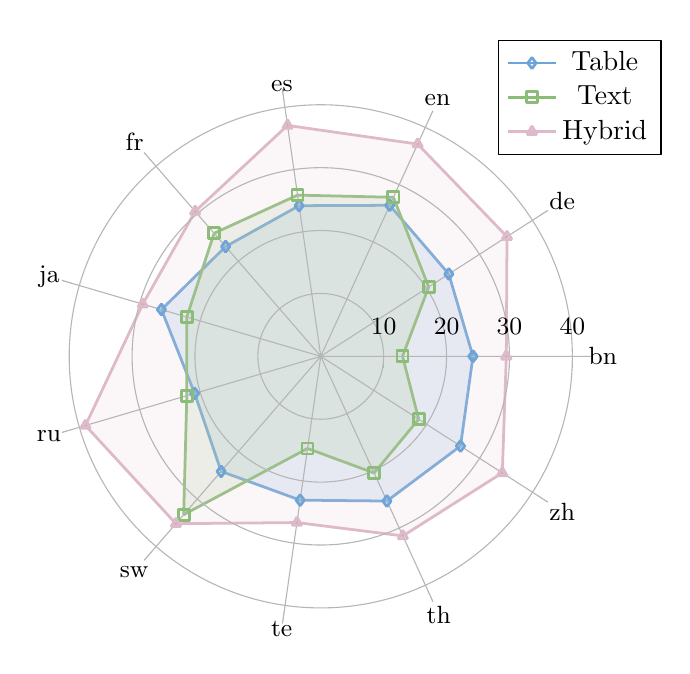
\begin{tikzpicture}
\begin{polaraxis}[
    title={\empty},
    xlabel={\empty},
    ylabel={\empty},
    xtick={0,32.73,65.46,98.19,130.92,163.65,196.38,229.11,261.84,294.57,327.30},
    xticklabels={bn, de, en, es, fr, ja, ru, sw, te, th, zh},
    % xticklabel style={font=\small, yshift=2ex}, % 标签离圆圈远一些,调整 y 轴偏移
    ytick={10,20,30,40},
    yticklabels={10,20,30,40},
    grid=both,
    tick label style={font=\small},
    major grid style={solid, gray}, % 外层圆圈设为黑色实线
    minor grid style={solid, gray}, % 次要网格线也设为黑色实线(可选)
    % axis line style={solid, black},   % 径向线设为灰色实线
    axis line style={draw=none},
    axis on top=true,                % 确保轴线在顶部
    grid style={gray},              % 确保网格线颜色为黑色
    line join=bevel,
    tick align=outside,
    % major grid style={solid, gray},
    % minor grid style={dotted, gray},
    % axis line style={draw=none},
    % axis on top
]

% 第一组数据
\addplot[
    color=data_blue!300,
    mark=diamond,
    style={line width=1pt},
    fill=data_blue!250,fill opacity=0.2
] coordinates {
    (0,24.2)(32.73,24.2)(65.46,26.4)(98.19,24.2)(130.92,23.1)(163.65,26.4)(196.38,20.9)(229.11,24.2)(261.84,23.1)(294.57,25.3)(327.30,26.4)(0,24.2)
} -- cycle;

% 第二组数据
\addplot[
    color=reasoner_green!300,
    mark=square,
    style={line width=1pt},
    fill=reasoner_green!250,fill opacity=0.2
] coordinates {
    (0,13.0)(32.73,20.4)(65.46,27.8)(98.19,25.9)(130.92,25.9)(163.65,22.2)(196.38,22.2)(229.11,33.3)(261.84,14.8)(294.57,20.4)(327.30,18.5)(0,13.0)
} -- cycle;


% 第三组数据
\addplot[
    color=annotator_pink!150,
    mark=triangle,
    style={line width=1pt},
    fill=annotator_pink,fill opacity=0.2
] coordinates {
    (0,29.5)(32.73,35.2)(65.46,37.1)(98.19,37.1)(130.92,30.5)(163.65,29.5)(196.38,39.0)(229.11,35.2)(261.84,26.7)(294.57,31.4)(327.30,34.3)(0,29.5)
} -- cycle;

\legend{Table, Text, Hybrid}

\end{polaraxis}
\end{tikzpicture}
}

%     \vspace{-0.5em}
%     \caption{
%         The EM of \ourmethod across different answer sources on Llama3.1-70B.
%     }
%     \label{fig:answer_source}
%     \vspace{-1em}
% \end{figure*}

\begin{figure}[t]
    \centering
    \resizebox{0.75\linewidth}{!}{
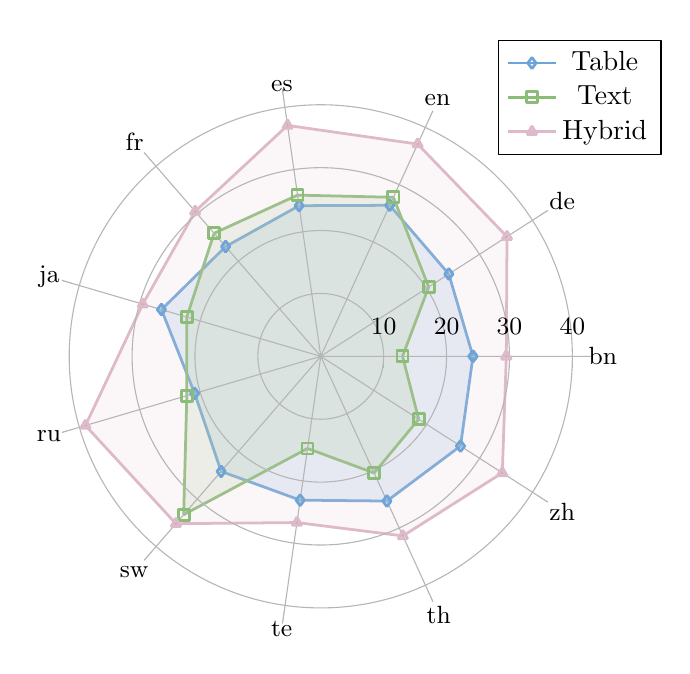
\begin{tikzpicture}
\begin{polaraxis}[
    title={\empty},
    xlabel={\empty},
    ylabel={\empty},
    xtick={0,32.73,65.46,98.19,130.92,163.65,196.38,229.11,261.84,294.57,327.30},
    xticklabels={bn, de, en, es, fr, ja, ru, sw, te, th, zh},
    % xticklabel style={font=\small, yshift=2ex}, % 标签离圆圈远一些,调整 y 轴偏移
    ytick={10,20,30,40},
    yticklabels={10,20,30,40},
    grid=both,
    tick label style={font=\small},
    major grid style={solid, gray}, % 外层圆圈设为黑色实线
    minor grid style={solid, gray}, % 次要网格线也设为黑色实线(可选)
    % axis line style={solid, black},   % 径向线设为灰色实线
    axis line style={draw=none},
    axis on top=true,                % 确保轴线在顶部
    grid style={gray},              % 确保网格线颜色为黑色
    line join=bevel,
    tick align=outside,
    % major grid style={solid, gray},
    % minor grid style={dotted, gray},
    % axis line style={draw=none},
    % axis on top
]

% 第一组数据
\addplot[
    color=data_blue!300,
    mark=diamond,
    style={line width=1pt},
    fill=data_blue!250,fill opacity=0.2
] coordinates {
    (0,24.2)(32.73,24.2)(65.46,26.4)(98.19,24.2)(130.92,23.1)(163.65,26.4)(196.38,20.9)(229.11,24.2)(261.84,23.1)(294.57,25.3)(327.30,26.4)(0,24.2)
} -- cycle;

% 第二组数据
\addplot[
    color=reasoner_green!300,
    mark=square,
    style={line width=1pt},
    fill=reasoner_green!250,fill opacity=0.2
] coordinates {
    (0,13.0)(32.73,20.4)(65.46,27.8)(98.19,25.9)(130.92,25.9)(163.65,22.2)(196.38,22.2)(229.11,33.3)(261.84,14.8)(294.57,20.4)(327.30,18.5)(0,13.0)
} -- cycle;


% 第三组数据
\addplot[
    color=annotator_pink!150,
    mark=triangle,
    style={line width=1pt},
    fill=annotator_pink,fill opacity=0.2
] coordinates {
    (0,29.5)(32.73,35.2)(65.46,37.1)(98.19,37.1)(130.92,30.5)(163.65,29.5)(196.38,39.0)(229.11,35.2)(261.84,26.7)(294.57,31.4)(327.30,34.3)(0,29.5)
} -- cycle;

\legend{Table, Text, Hybrid}

\end{polaraxis}
\end{tikzpicture}
}

    \caption{
        The EM of \ourmethod across different answer sources on \ourdataset using Llama3.1-70B.
    }
    \label{fig:answer_source}
\end{figure}

\paragraph{Answer Source}
% 我们分析了我们的方法使用Llama3.1-70B时在不同答案来源上的性能,如图所示
We analyze the performance of \ourmethod using Llama3.1-70B across different answer sources, as shown in Figure~\ref{fig:answer_source}. 
% 使用其他模型时以及不同的基线在不同来源上的性能在附录中提供
The performance with other models and baselines across answer sources is provided in Appendix~\ref{subsec:appendix_answer_source}. 
% 可以发现
The results show that:
% 1. 答案来源为Hybrid的问题的性能整体上优于单一答案来源的问题
(\emph{i})~The performance of the hybrid answer source generally outperforms those with a single answer source. 
% 因为我们的方法相比基线(见表)可以同时从表格和文本中链接到相关信息,整合了异质的相关上下文,一定程度上缓解了混合的答案来源的挑战
Since \ourmethod, compared to other baselines (see Figure~\ref{fig:answer_sources_other_baselines}), enhances the links between the question and the context, integrating hybrid contextual information and alleviating the challenge.
% 2. 虽然整体上英语的性能最佳,但在不同的答案来源上不同语言展现出了不同的趋势
% While English performs best overall, different languages exhibit varying trends across answer sources. 
% 不同语言在答案来源上的性能除了与高资源或低资源有关,还与语言本身的特性有关
(\emph{ii})~The performance across answer sources is influenced not only by the availability of language-specific resources but also by the characteristics of the language.
% 比如,词法结构复杂的语言在答案来源是text上的性能较差,如德语、俄语等
For instance, languages with complex morphological structures, such as German and Russian, perform worse when the answer source is text. 
% 而斯瓦希里语在文本上的性能最高,因为其有着较为简单的词法结构,能相对容易地根据问题中的实体链接到文本中的实体
In contrast, Swahili shows the highest performance on text-based sources, as its simpler morphology allows for easier linking of entities in the text to those in question \cite{tuan-nguyen-etal-2020-Vietnamese,zhang-etal-2023-xsemplr}.

% \begin{figure*}[t]
%     \centering
%     \resizebox{0.75\linewidth}{!}{
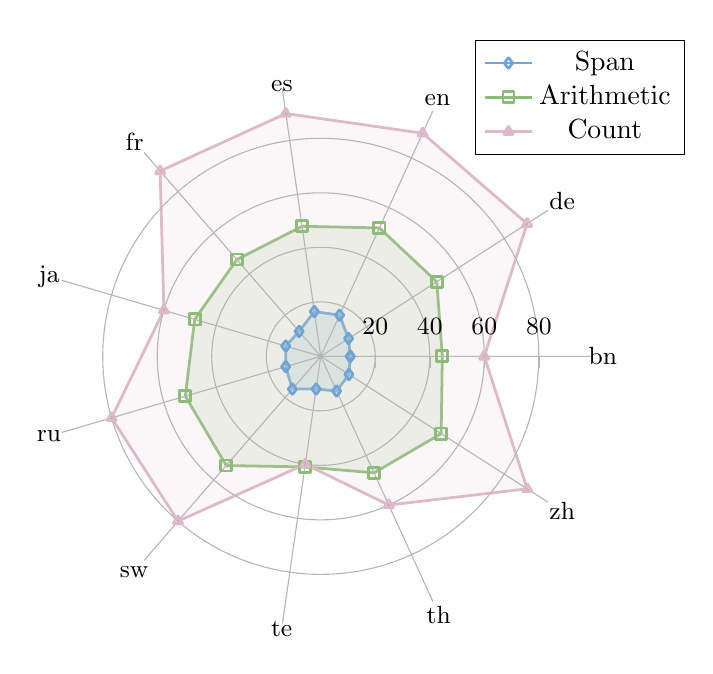
\begin{tikzpicture}
\begin{polaraxis}[
    title={\empty},
    xlabel={\empty},
    ylabel={\empty},
    xtick={0,32.73,65.46,98.19,130.92,163.65,196.38,229.11,261.84,294.57,327.30},
    xticklabels={bn, de, en, es, fr, ja, ru, sw, te, th, zh},
    % xticklabel style={font=\small, yshift=2ex}, % 标签离圆圈远一些,调整 y 轴偏移
    ytick={20,40,60,80,100},
    yticklabels={20,40,60,80,100},
    grid=both,
    tick label style={font=\small},
    major grid style={solid, gray}, % 外层圆圈设为黑色实线
    minor grid style={solid, gray}, % 次要网格线也设为黑色实线(可选)
    % axis line style={solid, black},   % 径向线设为灰色实线
    axis line style={draw=none},
    axis on top=true,                % 确保轴线在顶部
    grid style={gray},              % 确保网格线颜色为黑色
    line join=bevel,
    tick align=outside,
    % major grid style={solid, gray},
    % minor grid style={dotted, gray},
    % axis line style={draw=none},
    % axis on top
]

% 第一组数据
\addplot[
    color=data_blue!300,
    mark=diamond,
    style={line width=1pt},
    fill=data_blue!250,fill opacity=0.2
] coordinates {
    (0,10.8)(32.73,12.1)(65.46,16.6)(98.19,16.6)(130.92,12.1)(163.65,13.4)(196.38,13.4)(229.11,15.9)(261.84,12.1)(294.57,14.0)(327.30,12.3)(0,10.8)
} -- cycle;

% 第二组数据
\addplot[
    color=reasoner_green!300,
    mark=square,
    style={line width=1pt},
    fill=reasoner_green!250,fill opacity=0.2
] coordinates {
    (0,44.6)(32.73,50.6)(65.46,51.8)(98.19,48.2)(130.92,47.0)(163.65,48.2)(196.38,51.8)(229.11,53.0)(261.84,41.0)(294.57,47.0)(327.30,52.5)(0,44.6)
} -- cycle;

% 第三组数据
\addplot[
    color=annotator_pink!150,
    mark=triangle,
    style={line width=1pt},
    fill=annotator_pink,fill opacity=0.2
] coordinates {
    (0,60.0)(32.73,90.0)(65.46,90.0)(98.19,90.0)(130.92,90.0)(163.65,60.0)(196.38,80.0)(229.11,80.0)(261.84,40.0)(294.57,60.0)(327.30,90.0)(0,60.0)
} -- cycle;

\legend{Span, Arithmetic, Count}

\end{polaraxis}
\end{tikzpicture}
}

%     \vspace{-0.5em}
%     \caption{
%         The EM of \ourmethod across different answer types on Llama3.1-70B.
%     }
%     \label{fig:answer_type}
%     \vspace{-1em}
% \end{figure*}

\begin{figure}[t]
    \centering
    \resizebox{0.75\linewidth}{!}{
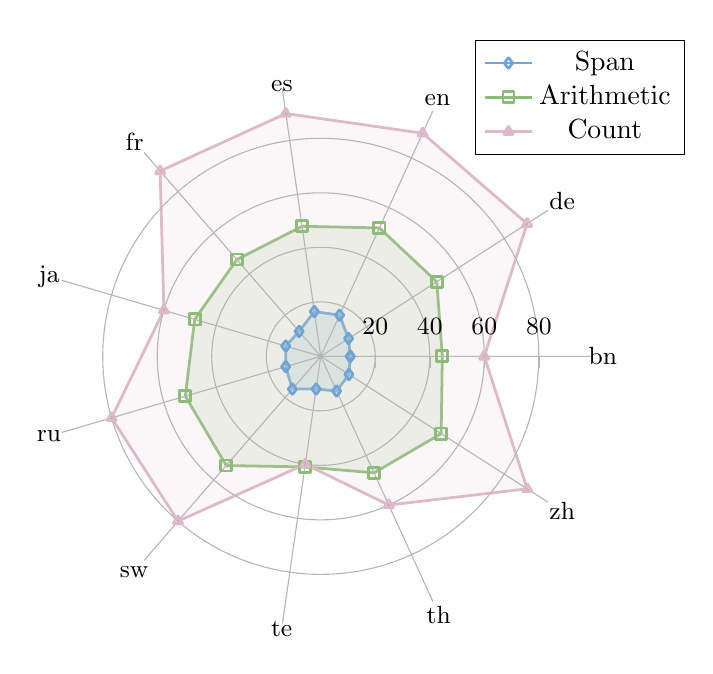
\begin{tikzpicture}
\begin{polaraxis}[
    title={\empty},
    xlabel={\empty},
    ylabel={\empty},
    xtick={0,32.73,65.46,98.19,130.92,163.65,196.38,229.11,261.84,294.57,327.30},
    xticklabels={bn, de, en, es, fr, ja, ru, sw, te, th, zh},
    % xticklabel style={font=\small, yshift=2ex}, % 标签离圆圈远一些,调整 y 轴偏移
    ytick={20,40,60,80,100},
    yticklabels={20,40,60,80,100},
    grid=both,
    tick label style={font=\small},
    major grid style={solid, gray}, % 外层圆圈设为黑色实线
    minor grid style={solid, gray}, % 次要网格线也设为黑色实线(可选)
    % axis line style={solid, black},   % 径向线设为灰色实线
    axis line style={draw=none},
    axis on top=true,                % 确保轴线在顶部
    grid style={gray},              % 确保网格线颜色为黑色
    line join=bevel,
    tick align=outside,
    % major grid style={solid, gray},
    % minor grid style={dotted, gray},
    % axis line style={draw=none},
    % axis on top
]

% 第一组数据
\addplot[
    color=data_blue!300,
    mark=diamond,
    style={line width=1pt},
    fill=data_blue!250,fill opacity=0.2
] coordinates {
    (0,10.8)(32.73,12.1)(65.46,16.6)(98.19,16.6)(130.92,12.1)(163.65,13.4)(196.38,13.4)(229.11,15.9)(261.84,12.1)(294.57,14.0)(327.30,12.3)(0,10.8)
} -- cycle;

% 第二组数据
\addplot[
    color=reasoner_green!300,
    mark=square,
    style={line width=1pt},
    fill=reasoner_green!250,fill opacity=0.2
] coordinates {
    (0,44.6)(32.73,50.6)(65.46,51.8)(98.19,48.2)(130.92,47.0)(163.65,48.2)(196.38,51.8)(229.11,53.0)(261.84,41.0)(294.57,47.0)(327.30,52.5)(0,44.6)
} -- cycle;

% 第三组数据
\addplot[
    color=annotator_pink!150,
    mark=triangle,
    style={line width=1pt},
    fill=annotator_pink,fill opacity=0.2
] coordinates {
    (0,60.0)(32.73,90.0)(65.46,90.0)(98.19,90.0)(130.92,90.0)(163.65,60.0)(196.38,80.0)(229.11,80.0)(261.84,40.0)(294.57,60.0)(327.30,90.0)(0,60.0)
} -- cycle;

\legend{Span, Arithmetic, Count}

\end{polaraxis}
\end{tikzpicture}
}

    \vspace{-0.5em}
    \caption{
        The EM of \ourmethod across different answer types on \ourdataset using Llama3.1-70B.
    }
    \label{fig:answer_type}
    \vspace{-1em}
\end{figure}

\paragraph{Answer Type}
% 我们比较了我们方法在Llama3.1-70B上在不同答案类型上的性能,如图所示
We compare the performance of \ourmethod using Llama3.1-70B on different answer types, as shown in Figure~\ref{fig:answer_type}. 
% 我们在附录提供了其他模型和基线在不同答案类型上的性能
Results of other models and baselines across answer types are provided in Appendix~\ref{subsec:appendix_answer_types}. 
% 我们发现
We observe that:
% 1. 模型在Span类型和Arithmetic上的性能不好,而在Count类型上的性能最高
% (\emph{i})~The model performs poorly on Span and Arithmetic types, while it performs best on the Count type. 
(\emph{i})~The model performs best on the Count type. 
% 因为span类型的答案需要从表格和文本中抽取出短语,或用几句话总结分析,相比较Arithmetic和Count的答案都为数字,对词语的构成和顺序更为敏感
This is because Span answers require extracting short phrases or summarizing conclusions from tables and text, making them more sensitive to word composition and order. 
% 而Arithmetic类型相比较Count类型需要模型进行更加复杂的运算
Additionally, Arithmetic answers involve more complex computations than Count answers.
% 2. 模型在不同答案类型上的性能整体上呈现高资源语言优于低资源语言
(\emph{ii})~The model performs better on high-resource languages than low-resource languages across answer types overall. 
% 即使我们的方法减小了性能差距,但低资源语言和高资源语言之间仍在不同的答案类型上均存在较大的性能差距
Although \ourmethod narrows the performance gap, there remains a significant difference between high-resource and low-resource languages for all answer types.

\subsection{Analysis}
% 在本小节,我们主要分析模型在TATQA任务上的跨语言能力

\begin{table*}[ht]
\centering
\tiny
% \begin{tabular}{llcccccccccccc}
% \toprule
% \textbf{Instruction} & \textbf{Demo} & \textbf{bn} & \textbf{de} & \textbf{en} & \textbf{es} & \textbf{fr} & \textbf{ja} & \textbf{ru} & \textbf{sw} & \textbf{te} & \textbf{th} & \textbf{zh} & \textbf{Average} \\
% \midrule
% \multirow{3}{*}{Native} & Native & $20.0/\bm{23.8}$ & $28.4/\bm{33.9}$ & $28.4/\bm{33.8}$ & $29.2/\bm{35.8}$ & $29.2/\bm{34.0}$ & $27.6/\bm{30.1}$ & $27.6/\bm{31.7}$ & $\bm{32.0}/35.1$ & $20.4/\bm{24.2}$ & $25.2/\bm{28.3}$ & $28.8/\bm{37.4}$ & $27.0/\bm{31.7}$ \\
% & Multi & $22.0/\bm{24.6}$ & $\bm{30.0}/32.3$ & $30.4/\bm{35.4}$ & $30.4/\bm{35.0}$ & $28.4/\bm{31.6}$ & $26.0/\bm{27.6}$ & $26.4/\bm{28.8}$ & $28.8/\bm{30.7}$ & $24.4/\bm{26.3}$ & $24.4/\bm{26.7}$ & $24.8/\bm{30.7}$ & $26.9/\bm{30.0}$ \\
% & En & $20.8/\bm{24.4}$ & $29.2/\bm{33.6}$ & $28.4/\bm{33.8}$ & $24.8/\bm{30.6}$ & $27.2/\bm{32.0}$ & $24.0/\bm{22.8}$ & $28.4/\bm{31.8}$ & $29.2/\bm{31.6}$ & $19.6/\bm{22.3}$ & $21.2/\bm{23.5}$ & $24.4/\bm{30.7}$ & $24.9/\bm{28.8}$ \\
% \midrule
% \multirow{3}{*}{En} & Native & $\bm{27.6}/30.5$ & $28.6/\bm{30.3}$ & $28.4/\bm{33.8}$ & $29.6/\bm{34.1}$ & $25.2/\bm{29.6}$ & $25.6/\bm{28.3}$ & $29.2/\bm{33.0}$ & $30.0/\bm{33.6}$ & $28.0/\bm{31.4}$ & $26.8/\bm{34.1}$ & $27.6/\bm{31.5}$ \\
% & Multi & $26.4/\bm{28.9}$ & $27.2/\bm{29.9}$ & $\bm{30.4}/35.4$ & $30.8/\bm{34.1}$ & $29.6/\bm{32.2}$ & $29.2/\bm{31.7}$ & $30.0/\bm{32.6}$ & $30.0/\bm{33.6}$ & $27.2/\bm{29.8}$ & $27.2/\bm{31.2}$ & $28.8/\bm{34.1}$ & $\bm{28.8}/32.1$ \\
% & En & $24.0/\bm{26.3}$ & $28.0/\bm{31.3}$ & $31.2/\bm{35.3}$ & $29.2/\bm{34.1}$ & $26.8/\bm{31.1}$ & $26.8/\bm{29.4}$ & $28.8/\bm{33.5}$ & $30.8/\bm{34.7}$ & $22.8/\bm{25.9}$ & $26.8/\bm{30.5}$ & $28.0/\bm{34.9}$ & $27.6/\bm{31.6}$ \\
% \bottomrule
% \end{tabular}

% \begin{tabular}{llcccccc}
% \toprule
% \textbf{Instruction} & \textbf{Demo} & \textbf{bn} & \textbf{de} & \textbf{en} & \textbf{es} & \textbf{fr} & \textbf{ja}\\
% \midrule
% \multirow{3}{*}{Native} & Native & $20.0/23.8$ & $28.4/33.9$ & $28.4/33.8$ & $29.2/35.8$ & $29.2/\bm{34.0}$ & $27.6/30.1$ \\
% & Multi & $22.0/24.6$ & $\bm{30.0/32.3}$ & $30.4/\bm{35.4}$ & $30.4/\bm{35.0}$ & $28.4/\bm{31.6}$ & $26.0/27.6$ \\
% & En & $20.8/24.4$ & $29.2/33.6$ & $28.4/33.8$ & $24.8/30.2$ & $27.2/32.0$ & $24.0/22.8$ \\
% \midrule
% \multirow{3}{*}{En} & Native & $\bm{27.6/30.5}$ & $26.8/30.3$ & $28.4/33.8$ & $29.6/32.7$ & $25.2/29.6$ & $25.6/28.5$ \\
% & Multi & $26.4/28.9$ & $27.2/29.9$ & $30.4/\bm{35.4}$ & $\bm{30.8}/34.1$ & $\bm{29.6}/32.2$ & $\bm{29.2/31.7}$ \\
% & En & $24.0/26.3$ & $28.0/31.3$ & $\bm{31.2}/35.3$ & $29.2/34.6$ & $26.8/31.1$ & $26.8/29.4$ \\
% \bottomrule
% \end{tabular}

% \begin{tabular}{llcccccc}
% \toprule
% \textbf{Instruction} & \textbf{Demo} & \textbf{ru} & \textbf{sw} & \textbf{te} & \textbf{th} & \textbf{zh} & \textbf{Avg.} \\
% \midrule
% \multirow{3}{*}{Native} & Native & $27.6/31.7$ & $\bm{32.0/35.1}$ & $20.4/24.2$ & $25.2/28.3$ & $\bm{28.8/37.4}$ & $27.0/31.7$ \\
% & Multi & $26.4/28.8$ & $28.8/30.7$ & $24.4/26.3$ & $24.4/26.7$ & $24.8/30.7$ & $26.9/30.0$ \\
% & En & $28.4/31.8$ & $29.2/31.6$ & $19.6/22.3$ & $21.2/23.5$ & $24.4/30.7$ & $24.9/28.8$ \\
% \midrule
% \multirow{3}{*}{En} & Native & $29.2/33.0$ & $30.0/33.6$ & $26.0/28.8$ & $\bm{28.0/31.4}$ & $26.8/34.1$ & $27.6/31.5$ \\
% & Multi & $\bm{30.0}/32.6$ & $30.0/33.0$ & $\bm{27.2/29.8}$ & $27.2/31.2$ & $\bm{28.8}/34.7$ & $\bm{28.8/32.1}$ \\
% & En & $28.8/\bm{33.5}$ & $30.8/34.7$ & $22.8/25.9$ & $26.8/30.5$ & $28.0/34.9$ & $27.6/31.6$ \\
% \bottomrule
% \end{tabular}

\begin{tabular}{l|l|ccccccccccc|c}
\toprule
\textbf{Instruction} & \textbf{Demo} & \textbf{bn} & \textbf{de} & \textbf{en} & \textbf{es} & \textbf{fr} & \textbf{ja} & \textbf{ru} & \textbf{sw} & \textbf{te} & \textbf{th} & \textbf{zh} & \textbf{Avg.} \\
\midrule
\multirow{3}{*}{Native} & Native & $20.0$ & $28.4$ & $28.4$ & $29.2$ & $29.2$ & $27.6$ & $27.6$ & \bm{$32.0$} & $20.4$ & $25.2$ & \bm{$28.8$} & $27.0$ \\
& Multi & $22.0$ & \bm{$30.0$} & $30.4$ & $30.4$ & $28.4$ & $26.0$ & $26.4$ & $28.8$ & $24.4$ & $24.4$ & $24.8$ & $26.9$ \\
& En & $20.8$ & $29.2$ & $28.4$ & $24.8$ & $27.2$ & $24.0$ & $28.4$ & $29.2$ & $19.6$ & $21.2$ & $24.4$ & $24.9$ \\
\midrule
\multirow{3}{*}{En} & Native & \bm{$27.6$} & $26.8$ & $28.4$ & $29.6$ & $25.2$ & $25.6$ & $29.2$ & $30.0$ & $26.0$ & \bm{$28.0$} & $26.8$ & $27.6$ \\
& Multi & $26.4$ & $27.2$ & $30.4$ & \bm{$30.8$} & \bm{$29.6$} & \bm{$29.2$} & \bm{$30.0$} & $30.0$ & \bm{$27.2$} & $27.2$ & \bm{$28.8$} & \bm{$28.8$} \\
& En & $24.0$ & $28.0$ & \bm{$31.2$} & $29.2$ & $26.8$ & $26.8$ & $28.8$ & $30.8$ & $22.8$ & $26.8$ & $28.0$ & $27.6$ \\
\bottomrule
\end{tabular}

\begin{tabular}{l|l|ccccccccccc|c}
\toprule
\textbf{Instruction} & \textbf{Demo} & \textbf{bn} & \textbf{de} & \textbf{en} & \textbf{es} & \textbf{fr} & \textbf{ja} & \textbf{ru} & \textbf{sw} & \textbf{te} & \textbf{th} & \textbf{zh} & \textbf{Avg.} \\
\midrule
\multirow{3}{*}{Native} & Native & $23.8$ & \bm{$33.9$} & $33.8$ & \bm{$35.8$} & $\bm{34.0}$ & $30.1$ & $31.7$ & \bm{$35.1$} & $24.2$ & $28.3$ & \bm{$37.4$} & $31.7$ \\
& Multi & $24.6$ & $32.3$ & $\bm{35.4}$ & $35.0$ & $31.6$ & $27.6$ & $28.8$ & $30.7$ & $26.3$ & $26.7$ & $30.7$ & $30.0$ \\
& En & $24.4$ & $33.6$ & $33.8$ & $30.2$ & $32.0$ & $22.8$ & $31.8$ & $31.6$ & $22.3$ & $23.5$ & $30.7$ & $28.8$ \\
\midrule
\multirow{3}{*}{En} & Native & \bm{$30.5$} & $30.3$ & $33.8$ & $32.7$ & $29.6$ & $28.5$ & $33.0$ & $33.6$ & $28.8$ & \bm{$31.4$} & $34.1$ & $31.5$ \\
& Multi & $28.9$ & $29.9$ & $\bm{35.4}$ & $34.1$ & $32.2$ & $\bm{31.7}$ & $32.6$ & $33.0$ & \bm{$29.8$} & $31.2$ & $34.7$ & \bm{$32.1$} \\
& En & $26.3$ & $31.3$ & $35.3$ & $34.6$ & $31.1$ & $29.4$ & $\bm{33.5}$ & $34.7$ & $25.9$ & $30.5$ & $34.9$ & $31.6$ \\
\bottomrule
\end{tabular}


\caption{
EM (above) and F1 (below) of \ourmethod using the instructions and demonstrations of different languages on Llama3.1-70B.
The best results under each language are annotated in \textbf{bold}. 
% Multi指的是由多种语言(英语、西班牙语和中文)组成的示例
Demo refers to demonstrations. 
Multi refers to demonstrations composed of multiple languages (English, Spanish, and Chinese).
Avg. denotes the average performance of the baseline across all languages.
}
\label{tab:prompt_language}
\end{table*}

% prompt的语言如何影响我们方法的性能
% How does the language of prompt affect the performance of our method?
% \subsubsection{Prompt Language}
\subsubsection{How does the Prompt Language Affect \ourmethod?}
% 我们分析了使用不同语言的instruction和示例对我们方法性能的影响,如表所示
We analyze the impact of using instructions and demonstrations in different languages on the performance of \ourmethod, as shown in Table~\ref{tab:prompt_language}. 
% 其中,多语言示例我们选择了分别是英语、西班牙语和中文的各一个示例,因为模型在这三个高资源语言上的性能较高,且包含两个语系
For the multilingual demonstrations, we select one demonstration each from English, Spanish, and Chinese, as the models perform well on these three high-resource languages, which also cover two language families. 
% 而英文instruction和英文示例是我们主实验采用的设置
The English instruction and English demonstrations are the settings of \ourmethod used in the main experiments. 
% 可以发现,
The results indicate that:


% 1. 使用英文instruction整体上优于使用原语言instruction
(\emph{i})~Using English instructions generally outperforms using native instructions.
% 2. 使用多语言示例打败了原语言和英语示例,说明当在某些语言上没有足够的TATQA示例时,可以采用同一语系或高资源语言的示例来提升模型性能
(\emph{ii})~Multilingual demonstrations outperform both native language and English demonstrations, suggesting that when sufficient native demonstrations are not available on the TATQA task, using demonstrations from the same language family or high-resource languages can also enhance performance.
% 同时,斯瓦希里语在使用原语言的instruction和示例时达到最高性能,说明了这种语言的独特性,模型不容易将在高资源语言上的知识和推理能力迁移到斯瓦西里语上
Additionally, Swahili achieves the highest performance when using instructions and examples in the native language, highlighting its uniqueness. 
% This suggests that it is difficult for the model to transfer knowledge and reasoning capabilities from high-resource languages to Swahili.

\begin{figure}[t]
    \centering
    \includegraphics[width=0.95\linewidth]{fig/heatmap_cross.pdf}
    \caption{
    % 被各个表示正确解决的instance之间的重复率
    The EM/F1 of \ourmethod with questions and context (table and text) of different languages on \ourdataset using Llama3.1-70B. 
    }
    \label{fig:heatmap_cross}
\end{figure}

% 跨语言
% \subsubsection{Cross-lingual QA}
\subsubsection{How does the Language Affect \ourmethod in the Cross-lingual Setting?}
% 我们评测了在跨语言QA,即问题和文本、表格的语言不一致的设置下我们的方法在我们数据集上的性能,如图所示
We evaluate the performance of \ourmethod in the cross-lingual setting, where the languages of the question and context are inconsistent, with results in Figure~\ref{fig:heatmap_cross}. 
% 我们分别选取了高资源语言法语和中文,以及低资源语言孟加拉语、斯瓦希里语和泰卢固语,涉及4个语系
We select high-resource languages (French and Chinese), and low-resource languages (Bengali, Swahili, and Telugu), covering $4$ language families. 
% 我们发现
Our findings include:
% 1. 普遍来讲,模型从低资源跨到高资源时会带来性能提升,反过来则下降
(\emph{i})~Generally, \ourmethod shows improved performance when transitioning from low-resource to high-resource languages, while the opposite results in a decline. 
% 比如用法语和中文对法语上下文提问的性能较高,而用三种低资源语言提问的性能较低
For instance, the performances on the French context with French and Chinese questions are relatively high, whereas the performances with three low-resource languages are lower.
% 2. 斯瓦希里语在跨语言的设置上表现出较为稳定的性能,且在同语言QA上达到最佳性能
(\emph{ii})~The model achieves the best performance when the question and context are both Swahili. 
% 因为斯瓦希里语较为规则的语法和词法结构,使其在我们的任务上受益,尤其是需要链接相关信息时相比其他语言更加容易
This can be attributed to its relatively regular grammatical and lexical structures, which provide advantages when linking related information.
% making it easier compared to other languages.

% \begin{table*}[ht]
% \centering
% \small
% 
\begin{lemma}\label{Lemma:multi1} 
   Fixing the number of data contributor $i$ collects $n_i$, and others' strategies $\strategy_{-i}$, $\hat{\mu}\left(X_i\right)$ is the minimax estimator for the Normal distribution class $\Normaldistrib := \left\{\mathcal{N}(\mu,\sigma^2) \;\middle|\; \mu \in \mathbb{R}\right\}$,
    \begin{align*}
       \hat{\mu}(X_i)  = \underset{\hat{\mu}}{\arg\min} \sbr{\sup _\mu \mathbb{E}\left[(\hat{\mu}( Y_i)- \hat{\mu}( Y_{-i}) )^2 \;\middle|\;  \mu \right] }
    \end{align*} 
     
\end{lemma}


\begin{proof}

\begin{align*}
    & \ \mathbb{E}\left[ \left( \hat{\mu}\left( Y_i \right)-\hat{\mu}\left( Y_{-i} \right)  \right)^2 \right] \\ =  & \ \mathbb{E}\left[ \left( (\hat{\mu}\left(  Y_i \right)-\mu) -(\hat{\mu}\left(  Y_{-i} \right) -\mu) \right)^2   \right] \\ =  & \ A_0 + \mathbb{E}\left[ (\hat{\mu}\left(  Y_i \right)-\mu)^2  \right]
\end{align*}
where $A_0$ is a positive coefficient.

Thus the maximum risk can be written as:

\begin{align*}
    \sup _\mu \mathbb{E}\left[A_0 + \left(\hat{\mu}\left( Y_i\right)-\mu\right)^{2} \;\middle|\;  \mu \right]
\end{align*}


We construct a lower bound on the maximum risk using a sequence of Bayesian risks. Let $\Lambda_{\ell}:=\mathcal{N}\left(0, \ell^2\right), \ell=1,2, \ldots$ be a sequence of prior for $\mu$. For fixed $\ell$, the posterior distribution is:
$$
\begin{aligned}
p\left(\mu \;\middle|\;  X_i\right) & \propto p\left(X_i \;\middle|\;  \mu\right) p(\mu) \\ & \propto \exp \left(-\frac{1}{2 \sigma^2} \sum_{x \in X_i}(x-\mu)^2\right) \exp \left(-\frac{1}{2 \ell^2} \mu^2\right) \\
& \propto \exp \left(-\frac{1}{2}\left(\frac{n_i}{\sigma^2}+\frac{1}{\ell^2}\right) \mu^2+\frac{1}{2} 2 \frac{\sum_{x \in X_i} x}{\sigma^2} \mu\right) .
\end{aligned}
$$

This means the posterior of $\mu$ given $X_i$ is Gaussian with:

\begin{align*}
    \mu \lvert\, X_i & \sim \mathcal{N}\left(\frac{n_i \hat{\mu}\left(X_i\right) / \sigma^2}{n_i / \sigma^2+1 / \ell^2}, \frac{1}{n_i / \sigma^2+1 / \ell^2}\right) 
    \\ & =: \mathcal{N}\left(\mu_{\ell}, \sigma_{\ell}^2\right).
\end{align*}



Therefore, the posterior risk is: 
$$
\begin{aligned}
&   \mathbb{E}\left[A_0 + \left(\hat{\mu}\left( Y_i\right)-\mu\right)^{2}  \;\middle|\;  X_i\right] \\ = &  \mathbb{E}\left[A_0 +  \left(\left(\hat{\mu}\left( Y_i\right)-\mu_{\ell}\right)-\left(\mu-\mu_{\ell}\right)\right)^{2 j} \;\middle|\;  X_i\right] \\ =
& A_0+\int_{-\infty}^{\infty} \underbrace{\left(e-\left(\hat{\mu}\left( Y_i\right)-\mu_{\ell}\right)\right)^2}_{=: F_1\left(e-\left(\hat{\mu}\left(Y_i\right)-\mu_{\ell}\right)\right)} \underbrace{\frac{1}{\sigma_{\ell} \sqrt{2 \pi}} \exp \left(-\frac{e^2}{2 \sigma_{\ell}^2}\right)}_{=: F_2(e)} d e
\end{aligned}
$$

Because:
\begin{itemize}
    \item $F_1(\cdot)$ is even function and increases on $[0, \infty)$;
    \item $F_2(\cdot)$ is even function and decreases on $\left[0, \infty \right)$, and $\int_{\mathbb{R}} F_2(e) de<\infty$
    \item For any $a \in \mathbb{R}, \int_{\mathbb{R}} F_1(e-a) F_2(e) de<\infty$
\end{itemize}

By the corollary of Hardy-Littlewood inequality in Lemma \ref{lemmaHardy},
$$
\int_{\mathbb{R}} F_1(e-a) F_2(e) d e \geq \int_{\mathbb{R}} F_1(e) F_2(e) d e
$$
which means the posterior risk is minimized when $\hat{\mu}\left(Y_i\right)=\mu_{\ell}$. We then write the Bayes risk as, the Bayes risk is minimized by the posterior mean $\mu_{\ell}$:

\begin{align*}    
R_{\ell}:= & \mathbb{E}\left[ A_0+\mathbb{E}\left[\left(\mu-\mu_{\ell}\right)^{2 } \;\middle|\;  X_i\right]\right] \\ = & A_0 + \sigma_{\ell}^{2}
\end{align*}

and the limit of Bayesian risk as $\ell \rightarrow \infty$ is
$$
R_{\infty}:= A_0 + \frac{\sigma^{2}}{n_i}.
$$

When $\hat{\mu}\left(Y_i\right)=\hat{\mu}\left(X_i\right)$, i.e, the contributor submit a set of size $n_i$ with each element equal to $ \hat{\mu}\left(X_i\right)$, the maximum risk is:

\begin{align*}
& \sup _\mu \mathbb{E}\left[A_0+\left(\mu- 
\hat{\mu}\left(Y_i\right) \right)^{2 } \;\middle|\;  \mu \right] \\
= & \sup _\mu \mathbb{E}\left[A_0+\left(\mu- 
\hat{\mu}\left(X_i\right) \right)^{2 } \;\middle|\;  \mu \right]  \\
= & A_0+ \sigma^{2 } n_i^{-1}  \\
= &  R_{\infty}.
\end{align*}

This implies that,
\begin{align*}
    & \underset{\mu}{\sup}\; \mathbb{E} \sbr{ \rbr{\hat{\mu}\left( Y_i \right)-\hat{\mu}\left( Y_{-i} \right)  }^2 \;\middle|\;  \mu }  \\ \geq & \; R_{\infty} =  \sup _\mu \; \mathbb{E}\left[A_0+\left(\mu- 
\hat{\mu}\left(X_i\right) \right)^{2 } \;\middle|\;  \mu \right]
\end{align*}

Therefore, the recommended strategy $\hat{\mu}(Y_i) =\hat{\mu}( X_i)$ has a smaller maximum risk than other strategies. 

\end{proof}




1. The payment from the buyer a constant $v(n^{\star})$.


2. If the payment for every seller is a fixed constant, then sellers can fabricate data without actually collecting data.\\


%$p_1 = b/2 +(\hat{\mu}(Y_1)- \hat{\mu}(Y_2))^2$, $p_2 = b/2 -(\hat{\mu}(Y_1)- \hat{\mu}(Y_2))^2$, seller 1 can choose ${\mu}' = u + \epsilon$, expected payment for seller 1 is larger than $b/2$. %NIC for seller 1: $g({\mu}',\mu ) < b/2$ for all ${\mu}' \neq \mu$. NIC for seller 2: $g( \mu, {\mu}') >  b/2 $ for all ${\mu}' \neq \mu$.

To demonstrate that no truthful mechanism (NIC) satisfies all desired properties in a two-seller setting, we use proof by contradiction.  

Suppose that there is a NIC mechanism $M$ satisfying property 1-5. Under this mechanism, the best strategy for each seller is to collect $N_i^{\star}$ amount of data and submit truthfully, where $N_1^{\star}+N_2^{\star} = n^{\star} $. Since $M$ is NIC for strategy space $\left\{ (f_i,N_i)\right\}_{i=1,2}$, it must be NIC for the sub strategy space $\left\{ (f_i, N_i^{\star})\right\}_{i=1,2}$. 


Consider the case in which everyone collects $N_i^{\star}$ data point and submits $N_i^{\star}$ data point. Assume that the true mean is $\mu$, seller $1$ submit $N({\mu}', \sigma^2),\ {\mu}' = f(\mu) $ while seller 2 submit $N({\mu}, \sigma^2) $. We denote seller 1's expected payment as  $\mathbb{E}\left[ p_1(M,\strategy) \right] = g({\mu}', \mu)$.
Seller 1's utility is then:
\[ u_1(M,f) = \underset{\mu}{\inf} \ g({\mu}', \mu) -c\times N_1^{\star}\] where $c$ is the cost for collecting one data point.


The total payment from the buyer is $v(n^{\star})$, hence by budget balance, \[p_2 (M,f)  = v(n^{\star}) -  p_1(M,f), \ \mathbb{E}\left[ p_2(M,f) \right] = v(n^{\star}) - g({\mu}', \mu) \]

By NIC, we have,
\[ \underset{\mu}{\inf} \ g({\mu}', \mu) -c\times N_1^{\star} \leq \underset{\mu}{\inf} \ g({\mu}, \mu) -c\times N_1^{\star} \] \[ \underset{\mu}{\inf} \ (v(n^{\star})- g( \mu, {\mu}')) -c\times N_2^{\star} \leq \underset{\mu}{\inf} \ (v(n^{\star})-g( \mu, {\mu})) -c\times N_2^{\star}  \]

%Using the fact that $\underset{\mu}{\inf} \ g({\mu}, \mu) = \underset{\mu}{\sup} \ g({\mu}, \mu) = {v(n^{\star})}/2 $.
We obtain that for any ${\mu}'$ and $\mu$,
\[  \underset{\mu}{\inf} \ g({\mu}', \mu) \leq \underset{\mu}{\inf} \ g({\mu}, \mu)   \] \[  \underset{\mu}{\sup} \  g( \mu, {\mu})  \leq \underset{\mu}{\sup } \ g( \mu, {\mu}')  \]

We next show that the inequalities are strict. Assume, for contradiction there exists ${\mu}'$, for any $\mu$, $g({\mu}', 
\mu) \geq \underset{\mu}{\inf} \ g({\mu}, \mu)$. It then follows that $ \underset{\mu}{\inf} \ g({\mu}', \mu) \geq \underset{\mu}{\inf} \ g({\mu}, \mu)$. Under this assumption, seller 1 could fabricate data by submitting $N({\mu}', \sigma^2)$ without collecting any actual data. This contradicts with the fact that $(f_1 = I, N_1 = N_1^{\star})$ is the best strategy for seller 1. Hence, for any ${\mu}'$, there exists some $\mu$ such that $g({\mu}', 
\mu) < \underset{\mu}{\inf} \ g({\mu}, \mu)$. Therefore, for any ${\mu}'$, \[ \underset{\mu}{\inf} \ g({\mu}', \mu) < \underset{\mu}{\inf} \ g({\mu}, \mu). \]Similarly, we also have \[ \underset{\mu}{\sup} \  g( \mu, {\mu})  < \underset{\mu}{\sup } \ g( \mu, {\mu}').  \] 


For any $ {\mu}'$, let $f({\mu}') =  \underset{\mu}{\arg\sup}\, g(\mu, {\mu}')$, then we have for any ${\mu}'$,  $f({\mu}') \neq {\mu}'$ and $ g(f({\mu}'), {\mu}') > \underset{\mu}{\sup} \  g( \mu, {\mu}) \geq  \underset{\mu}{\inf} \  g( \mu, {\mu})$. This implies that seller 1 could fabricate data based on function $f$, this contradicts with the fact that the mechanism is NIC.


pay the seller $v(n^{\star})/2 - \beta (\hat{\mu}(Y_1)-\hat{\mu}(Y_2))^2$, charge buyer $v(n^{\star}) - 2\beta (\hat{\mu}(Y_1)-\hat{\mu}(Y_2))^2$


Buyer utility: $v(n^*)$-payment
Seller utility: payment - $cn^*$.

Sellers utility is positive?

Seller payment $(v(n^*)/2)-\beta (\hat{\mu}(Y_1)-\hat{\mu}(Y_2))^2 $, $\beta = (v(n^*)-cn^*)c(n^*)^2 / 4\sigma^2$, 



\section{Multiple buyers}
\subsection{}
Question 1: Do we fix the amount of data for sale ahead of time?


Assume we fix $N$, the amount of data for sale. The goal of mechanism is to maximize the sellers' revenue. According to previous paper, there exists at least one type who purchase at the amount $N$. Suppose that in offline setting, i.e., when the mechanism knows the buyer valuation and type distribution, the optimal revenue is $\text{OPT} $. 


We ask $d$ sellers to collect $N$ data points, and split $\text{OPT} $ revenue among sellers. (data can be duplicated). 

\[ p_i(M,s) =\mathbb{I}\left( \left| Y_i \right| = \frac{N}{d} \right) \rbr{\frac{\text{OPT}}{d}+d_i \frac{\sigma^2}{N_{-i}^{\star}} +d_i \frac{\sigma^2}{N_i^{\star}} }- d_i \rbr{\hat{\mu}(Y_i)-\hat{\mu}(Y_{-i}) }^2  \]

Buyer's expected utility is non negative. Next, we discuss sellers' expected utility $T\mathbb{E}[p_i]- cn_i$ (over $T$ roundsm\, maybe $T$ is fixed). Let $N_i^{\star} = \frac{N}{d}$.

\[ u_i(M,s) = \mathbb{I}\left( \left| Y_i \right| = \frac{N}{d} \right) \rbr{\frac{\text{OPT}}{d}+d_i \frac{\sigma^2}{N_{-i}^{\star}} +d_i \frac{\sigma^2}{N_i^{\star}} }T- Td_i \mathbb{E}\rbr{\hat{\mu}(Y_i)-\hat{\mu}(Y_{-i}) }^2 
 -  cn_i \]
Choose $d_i = \frac{c(N_i^{\star})^2}{T\sigma^2}$.


If we do not fix \( T \) in advance, let \( T_0 \) represent the time at which the cumulative utility over at least \( T_0 \) rounds is non-negative. We can select \( d_i \) such that \( d_i \geq \frac{c(N/d)^2}{T_0 \sigma^2} \). This ensures that the seller will never choose to collect less than \( N/d \) amount of data.








\section{Single buyer} \label{section: singlebuyer}


Each contributor \( i \) incurs a cost \( c_i \) to collect data,  without loss of generality, we assume \( c_1 \leq c_2 \leq \dots \leq c_d \). The broker is assumed to have full knowledge of the buyer's valuation curve \( \val(n) \), as well as the contributors’ costs $ c_{ i \in \contributors}$  for collecting each data point.

The maximum total profit for the contributors, assuming no constraints on truthful submissions, is given by:
\[
\mathrm{profit}^\star = \underset{\datanum_1, \dots, \datanum_d}{\max} \left( \val \left(\sum_{i=1}^{d} \datanum_i\right) - \sum_{i=1}^{d} c_i \datanum_i \right),
\]

where \( \datanum_i \) represents the number of data points collected by contributor \( i \). In this unconstrained scenario, since contributor 1 has the lowest collection cost, the optimal strategy is for contributor 1 to collect all the required data points while other contributors collect none. This approach maximizes total profit without considering the incentive for truthful submissions.

However, when truthful submission is taken into account, at least two contributors are needed because we need to use one contributor's data to verify the other's. We demonstrate that the maximum profit achievable under Nash Equilibrium is:
\[
\mathrm{profit}^\star + (c_1 - c_2),
\]
where \( c_1 - c_2 \) represents the additional cost differential caused by enforcing truthful behavior among contributors. 

\begin{algorithm}[H]
    \caption{Process of mechanism.}
    \begin{algorithmic}
        \STATE {\bfseries Input:} A population of buyers $\buyers$.
        \STATE The broker chooses the optimal data allocation to maximize contributors' profit:
        $$
        \{ \datanum_i^{\star} \}_{i=1}^d = \underset{\datanum_1,\dots,\datanum_d}{\arg\max}\  \rbr{v\rbr{\sum_i \datanum_i}-\sum_i \cost_i \datanum_i  }
      $$
       
        \STATE The broker recommend a strategy to each contributor: $\strategy_i^{\star} = (\datanum_i^{\star}, \mathbf{I})$.
        \STATE Each contributor selects a strategy $\strati = (\datanum_i, f_i)$, collects $\datanum_i$ data points $X_i$, and submits $Y_i = f_i(X_i)$.
        \STATE The mechanism generates an estimator $\hat{\mu}(M,\strategy)$ for the buyer, and charge her $\price_{j \in \buyers}$. \COMMENT{See (\ref{eq:buyer_pay}) }
        \STATE Each contributor is paid $\payi$.    \COMMENT{See (\ref{eq:seller_pay}) }
    \end{algorithmic}   
\end{algorithm}




\begin{theorem}
    there exists NIC mechanism satisfying the following properties (1) $\strategy^{\star}$ is Nash equilibrium. (2) The mechanism is individually rational at $\strategy^{\star}$ for both buyers and sellers. (3) Budget balance. (4) Under strategy $\strategy^{\star}$, the expected profit of buyers approximates the optimal profit $ \mathrm{profit}^{\star}$ within an additive error $\cost_2 - \cost_1$. 
\end{theorem}


Let $n^{\star}$ denote the optimal total number of data to be collected, $\datanum_1^{\star}=n^{\star}-1$, and $\datanum_2^{\star}=1$. Let $w=\val(n^{\star})-cn^{\star}$ denote the social welfare. One option for payment function is

\begin{align*}
    &\; \pay_i(M,\strategy^{\star}) \\  
    = & \;\mathbb{I}\left( \left| Y_i \right| = \datanum_i^{\star} \right) \rbr{\frac{\datanum_1^{\star}}{n^{\star}}\val(n^{\star})+d_i \frac{\sigma^2}{\datanum_{-i}^{\star}} +d_i \frac{\sigma^2}{\datanum_i^{\star}} } \\ & - d_i \rbr{\hat{\mu}(Y_i)-\hat{\mu}(Y_{-i}) }^2, \\[20pt] % Adds vertical space between equations
    &\; \price(M,\strategy^{\star}) \\  
    = & \; \sum_{i=1}^{2}\mathbb{I}\left(  \left| Y_i \right| = \datanum_i^{\star} \right) \rbr{\frac{\datanum_1^{\star}}{n^{\star}}\val(n^{\star}) +d_i \frac{\sigma^2}{\datanum_{-i}^{\star}} +d_i \frac{\sigma^2}{\datanum_i^{\star}} } \\ 
    & - \sum_{i=1}^{2} d_i \rbr{\hat{\mu}(Y_i)-\hat{\mu}(Y_{-i}) }^2, \\[20pt] % Adds vertical space between equations
    &\;  \utilityb (M,\strategy^{\star}) \\ 
   = & \; v(\datanum^{\star}) -\mathbb{E}[\price(M,\strategy^{\star})] \\ 
    = & \; - \sum_{i=1}^{d} \rbr{d_i \frac{\sigma^2}{\datanum_{-i}^{\star}} +d_i \frac{\sigma^2}{\datanum_i^{\star}}  } + \sum_{i=1}^{d}d_i \mathbb{E} \rbr{\hat{\mu}(Y_i)-\hat{\mu}(Y_{-i}) }^2 \\ 
    = & \; 0.
\end{align*}



Then contributors i's expected ptofit under strategy $\strategy^{\star}$ is 

\begin{align*}
& \; \utilci \rbr{\mechspace, \strategy^{\star} } \\ = &  \; \mathbb{E}\sbr{\pay_i(M,\strategy^{\star})} - \cost_i n_i^{\star} \\ = &  \; \mathbb{I}\left(\left| Y_i \right| = \datanum_i^{\star} \right) \rbr{\frac{\datanum_1^{\star}}{n^{\star}}\val(n^{\star})  +d_i \frac{\sigma^2}{\datanum_{-i}^{\star}} +d_i \frac{\sigma^2}{\datanum_i^{\star}} }\\  & -  d_i \mathbb{E}\rbr{\hat{\mu}(Y_i)-\hat{\mu}(Y_{-i}) }^2  -\cost n_i^{\star} \\ = &  \;  \frac{w}{\numcontributors}
\end{align*}
where $d_i = c(\datanum_i^*/d)^2 $, 

%\textcolor{red}{Buyer payment $\pi(M,s)$ can ve negative? Can it be interpreted as when the quality of data is bad, the mechanism pays money to the buyer as compensate, the contributor pays money to the mechanism as a penalty. }\textcolor{red}{Buyer pays $v(n^*)$, $p_i = v(n^*) \frac{\rbr{\hat{\mu}(Y_i)-\hat{\mu}(Y_{-i}) }^{-2}}{\sum{\rbr{\hat{\mu}(Y_i)-\hat{\mu}(Y_{-i}) }^{-2}}}$ }


We prove the NIC in three steps.


\textbf{First step} \textcolor{red}{to be fixed}: Giving others submitting truthfully, we know that when fixing $n_i$, submitting $\left| Y_i \right| = \frac{n^{\star}}{d}$ is the best strategy, otherwise, $\pay_i <0$ when $\left| Y_i \right| \neq \frac{n^{\star}}{d}$. Therefore, for any $n_i$ and $f_i$, we have for any $\mu$,
\begin{align*}
& u_i\rbr{\mechspace, (n_i,f_i, \left| Y_i \right| =\datanum_i^{\star}),\strategy_{-i}^{\star} } \\  \geq \  & u_i\rbr{\mechspace, \strategy_{-i}^{\star}} 
\end{align*}

\textbf{Second step}: Fixing $n_i$ and $\left| Y_i \right|$, sample mean $\hat{\mu}(X_i)$ is minimax estimator of $\mathbb{E}\rbr{\rbr{\hat{\mu}(Y_i)-\hat{\mu}(Y_{-i})}^2 \;\middle|\; P} $, i.e., \[ \hat{\mu}(X_i) = \underset{\hat{\mu}}{\inf} \  \underset{\distrifamily}{\sup}\ \mathbb{E}\sbr{\rbr{\hat{\mu}(Y_i)-\hat{\mu}(Y_{-i})}^2  \;\middle|\; \distri} \]Therefore we have 
\begin{align*}
     & \underset{\distrifamily}{\inf}\;u_i\rbr{\mechspace, (n_i,\hat{\mu}(Y_i)=\hat{\mu}(X_i), \left| Y_i \right|),\strategy_{-i}^{\star} } \\  \geq \  & \underset{\distrifamily}{\inf}\;u_i\rbr{\mechspace, (n_i,\hat{\mu}(Y_i), \left| Y_i \right|),\strategy_{-i}^{\star} } 
\end{align*}


\textbf{Third step}: By setting constant $d_i= c\rbr{\frac{\datanum_i^{\star}}{\sigma}}^2$, when fixing $\hat{\mu}(Y_i)=\hat{\mu}(X_i)$ and $\left| Y_i \right| = \datanum_i^{\star}$, collecting $n_i = \datanum_i^{\star}$ amount of data maximize the contributor utility 
\begin{align*}
    \underset{\distrifamily}{\inf}\;u_i\rbr{\mechspace, (n_i= \datanum_i^{\star},\hat{\mu}(Y_i)=\hat{\mu}(X_i), \left| Y_i \right|=\strategy_{-i}^{\star} } \\ \geq \underset{\distrifamily}{\inf}\;u_i\rbr{\mechspace, (n_i,\hat{\mu}(Y_i)=\hat{\mu}(X_i), \left| Y_i \right|=s_{-i}^{\star}}  
\end{align*}
 

\begin{align*}
    & u_i\rbr{\mechspace, (n_i,\hat{\mu}(Y_i)=\hat{\mu}(X_i), \left| Y_i \right|=\datanum_i^{\star}),\strategy_{-i}^{\star} }  \\ = & \rbr{\frac{w}{\numcontributors}+ c \datanum_i^{\star} +d_i \frac{\sigma^2}{\datanum_{-i}^{\star}} +d_i \frac{\sigma^2}{\datanum_i^{\star}} } - d_i \rbr{ \frac{\sigma^2}{\datanum_{-i}^{\star}} +\frac{\sigma^2}{\datanum_i^{\star}} } - cn_i
\end{align*}

Therefore, we have 
\begin{align*}
    &\underset{\distrifamily}{\inf}\;u_i \rbr{\mechspace, (n_i= \datanum_i^{\star},\hat{\mu}(Y_i)=\hat{\mu}(X_i), \left| Y_i \right|=\datanum_i^{\star}),\strategy_{-i}^{\star} } \\  = & \underset{\distrifamily}{\inf}\;u_i\rbr{\mechspace, (\datanum_i^{\star},f_i^{\star}),\strategy_{-i}^{\star} } \\ \geq &   \underset{\distrifamily}{\inf}\; u_i\rbr{\mechspace, (n_i,f_i ),\strategy_{-i}^{\star}} 
\end{align*}

When following the best strategy, properties 1-5 are all satisfied.



% \caption{
%     % 我们方法上非英语相比英语性能落后的错误原因,及比例
%     The error types and the proportion of non-English performance in \ourmethod are lagging behind that of English.
% }
% \label{tab:error}
% \end{table*}

\begin{figure}[t]
    \centering
    
\begin{lemma}\label{Lemma:multi1} 
   Fixing the number of data contributor $i$ collects $n_i$, and others' strategies $\strategy_{-i}$, $\hat{\mu}\left(X_i\right)$ is the minimax estimator for the Normal distribution class $\Normaldistrib := \left\{\mathcal{N}(\mu,\sigma^2) \;\middle|\; \mu \in \mathbb{R}\right\}$,
    \begin{align*}
       \hat{\mu}(X_i)  = \underset{\hat{\mu}}{\arg\min} \sbr{\sup _\mu \mathbb{E}\left[(\hat{\mu}( Y_i)- \hat{\mu}( Y_{-i}) )^2 \;\middle|\;  \mu \right] }
    \end{align*} 
     
\end{lemma}


\begin{proof}

\begin{align*}
    & \ \mathbb{E}\left[ \left( \hat{\mu}\left( Y_i \right)-\hat{\mu}\left( Y_{-i} \right)  \right)^2 \right] \\ =  & \ \mathbb{E}\left[ \left( (\hat{\mu}\left(  Y_i \right)-\mu) -(\hat{\mu}\left(  Y_{-i} \right) -\mu) \right)^2   \right] \\ =  & \ A_0 + \mathbb{E}\left[ (\hat{\mu}\left(  Y_i \right)-\mu)^2  \right]
\end{align*}
where $A_0$ is a positive coefficient.

Thus the maximum risk can be written as:

\begin{align*}
    \sup _\mu \mathbb{E}\left[A_0 + \left(\hat{\mu}\left( Y_i\right)-\mu\right)^{2} \;\middle|\;  \mu \right]
\end{align*}


We construct a lower bound on the maximum risk using a sequence of Bayesian risks. Let $\Lambda_{\ell}:=\mathcal{N}\left(0, \ell^2\right), \ell=1,2, \ldots$ be a sequence of prior for $\mu$. For fixed $\ell$, the posterior distribution is:
$$
\begin{aligned}
p\left(\mu \;\middle|\;  X_i\right) & \propto p\left(X_i \;\middle|\;  \mu\right) p(\mu) \\ & \propto \exp \left(-\frac{1}{2 \sigma^2} \sum_{x \in X_i}(x-\mu)^2\right) \exp \left(-\frac{1}{2 \ell^2} \mu^2\right) \\
& \propto \exp \left(-\frac{1}{2}\left(\frac{n_i}{\sigma^2}+\frac{1}{\ell^2}\right) \mu^2+\frac{1}{2} 2 \frac{\sum_{x \in X_i} x}{\sigma^2} \mu\right) .
\end{aligned}
$$

This means the posterior of $\mu$ given $X_i$ is Gaussian with:

\begin{align*}
    \mu \lvert\, X_i & \sim \mathcal{N}\left(\frac{n_i \hat{\mu}\left(X_i\right) / \sigma^2}{n_i / \sigma^2+1 / \ell^2}, \frac{1}{n_i / \sigma^2+1 / \ell^2}\right) 
    \\ & =: \mathcal{N}\left(\mu_{\ell}, \sigma_{\ell}^2\right).
\end{align*}



Therefore, the posterior risk is: 
$$
\begin{aligned}
&   \mathbb{E}\left[A_0 + \left(\hat{\mu}\left( Y_i\right)-\mu\right)^{2}  \;\middle|\;  X_i\right] \\ = &  \mathbb{E}\left[A_0 +  \left(\left(\hat{\mu}\left( Y_i\right)-\mu_{\ell}\right)-\left(\mu-\mu_{\ell}\right)\right)^{2 j} \;\middle|\;  X_i\right] \\ =
& A_0+\int_{-\infty}^{\infty} \underbrace{\left(e-\left(\hat{\mu}\left( Y_i\right)-\mu_{\ell}\right)\right)^2}_{=: F_1\left(e-\left(\hat{\mu}\left(Y_i\right)-\mu_{\ell}\right)\right)} \underbrace{\frac{1}{\sigma_{\ell} \sqrt{2 \pi}} \exp \left(-\frac{e^2}{2 \sigma_{\ell}^2}\right)}_{=: F_2(e)} d e
\end{aligned}
$$

Because:
\begin{itemize}
    \item $F_1(\cdot)$ is even function and increases on $[0, \infty)$;
    \item $F_2(\cdot)$ is even function and decreases on $\left[0, \infty \right)$, and $\int_{\mathbb{R}} F_2(e) de<\infty$
    \item For any $a \in \mathbb{R}, \int_{\mathbb{R}} F_1(e-a) F_2(e) de<\infty$
\end{itemize}

By the corollary of Hardy-Littlewood inequality in Lemma \ref{lemmaHardy},
$$
\int_{\mathbb{R}} F_1(e-a) F_2(e) d e \geq \int_{\mathbb{R}} F_1(e) F_2(e) d e
$$
which means the posterior risk is minimized when $\hat{\mu}\left(Y_i\right)=\mu_{\ell}$. We then write the Bayes risk as, the Bayes risk is minimized by the posterior mean $\mu_{\ell}$:

\begin{align*}    
R_{\ell}:= & \mathbb{E}\left[ A_0+\mathbb{E}\left[\left(\mu-\mu_{\ell}\right)^{2 } \;\middle|\;  X_i\right]\right] \\ = & A_0 + \sigma_{\ell}^{2}
\end{align*}

and the limit of Bayesian risk as $\ell \rightarrow \infty$ is
$$
R_{\infty}:= A_0 + \frac{\sigma^{2}}{n_i}.
$$

When $\hat{\mu}\left(Y_i\right)=\hat{\mu}\left(X_i\right)$, i.e, the contributor submit a set of size $n_i$ with each element equal to $ \hat{\mu}\left(X_i\right)$, the maximum risk is:

\begin{align*}
& \sup _\mu \mathbb{E}\left[A_0+\left(\mu- 
\hat{\mu}\left(Y_i\right) \right)^{2 } \;\middle|\;  \mu \right] \\
= & \sup _\mu \mathbb{E}\left[A_0+\left(\mu- 
\hat{\mu}\left(X_i\right) \right)^{2 } \;\middle|\;  \mu \right]  \\
= & A_0+ \sigma^{2 } n_i^{-1}  \\
= &  R_{\infty}.
\end{align*}

This implies that,
\begin{align*}
    & \underset{\mu}{\sup}\; \mathbb{E} \sbr{ \rbr{\hat{\mu}\left( Y_i \right)-\hat{\mu}\left( Y_{-i} \right)  }^2 \;\middle|\;  \mu }  \\ \geq & \; R_{\infty} =  \sup _\mu \; \mathbb{E}\left[A_0+\left(\mu- 
\hat{\mu}\left(X_i\right) \right)^{2 } \;\middle|\;  \mu \right]
\end{align*}

Therefore, the recommended strategy $\hat{\mu}(Y_i) =\hat{\mu}( X_i)$ has a smaller maximum risk than other strategies. 

\end{proof}




1. The payment from the buyer a constant $v(n^{\star})$.


2. If the payment for every seller is a fixed constant, then sellers can fabricate data without actually collecting data.\\


%$p_1 = b/2 +(\hat{\mu}(Y_1)- \hat{\mu}(Y_2))^2$, $p_2 = b/2 -(\hat{\mu}(Y_1)- \hat{\mu}(Y_2))^2$, seller 1 can choose ${\mu}' = u + \epsilon$, expected payment for seller 1 is larger than $b/2$. %NIC for seller 1: $g({\mu}',\mu ) < b/2$ for all ${\mu}' \neq \mu$. NIC for seller 2: $g( \mu, {\mu}') >  b/2 $ for all ${\mu}' \neq \mu$.

To demonstrate that no truthful mechanism (NIC) satisfies all desired properties in a two-seller setting, we use proof by contradiction.  

Suppose that there is a NIC mechanism $M$ satisfying property 1-5. Under this mechanism, the best strategy for each seller is to collect $N_i^{\star}$ amount of data and submit truthfully, where $N_1^{\star}+N_2^{\star} = n^{\star} $. Since $M$ is NIC for strategy space $\left\{ (f_i,N_i)\right\}_{i=1,2}$, it must be NIC for the sub strategy space $\left\{ (f_i, N_i^{\star})\right\}_{i=1,2}$. 


Consider the case in which everyone collects $N_i^{\star}$ data point and submits $N_i^{\star}$ data point. Assume that the true mean is $\mu$, seller $1$ submit $N({\mu}', \sigma^2),\ {\mu}' = f(\mu) $ while seller 2 submit $N({\mu}, \sigma^2) $. We denote seller 1's expected payment as  $\mathbb{E}\left[ p_1(M,\strategy) \right] = g({\mu}', \mu)$.
Seller 1's utility is then:
\[ u_1(M,f) = \underset{\mu}{\inf} \ g({\mu}', \mu) -c\times N_1^{\star}\] where $c$ is the cost for collecting one data point.


The total payment from the buyer is $v(n^{\star})$, hence by budget balance, \[p_2 (M,f)  = v(n^{\star}) -  p_1(M,f), \ \mathbb{E}\left[ p_2(M,f) \right] = v(n^{\star}) - g({\mu}', \mu) \]

By NIC, we have,
\[ \underset{\mu}{\inf} \ g({\mu}', \mu) -c\times N_1^{\star} \leq \underset{\mu}{\inf} \ g({\mu}, \mu) -c\times N_1^{\star} \] \[ \underset{\mu}{\inf} \ (v(n^{\star})- g( \mu, {\mu}')) -c\times N_2^{\star} \leq \underset{\mu}{\inf} \ (v(n^{\star})-g( \mu, {\mu})) -c\times N_2^{\star}  \]

%Using the fact that $\underset{\mu}{\inf} \ g({\mu}, \mu) = \underset{\mu}{\sup} \ g({\mu}, \mu) = {v(n^{\star})}/2 $.
We obtain that for any ${\mu}'$ and $\mu$,
\[  \underset{\mu}{\inf} \ g({\mu}', \mu) \leq \underset{\mu}{\inf} \ g({\mu}, \mu)   \] \[  \underset{\mu}{\sup} \  g( \mu, {\mu})  \leq \underset{\mu}{\sup } \ g( \mu, {\mu}')  \]

We next show that the inequalities are strict. Assume, for contradiction there exists ${\mu}'$, for any $\mu$, $g({\mu}', 
\mu) \geq \underset{\mu}{\inf} \ g({\mu}, \mu)$. It then follows that $ \underset{\mu}{\inf} \ g({\mu}', \mu) \geq \underset{\mu}{\inf} \ g({\mu}, \mu)$. Under this assumption, seller 1 could fabricate data by submitting $N({\mu}', \sigma^2)$ without collecting any actual data. This contradicts with the fact that $(f_1 = I, N_1 = N_1^{\star})$ is the best strategy for seller 1. Hence, for any ${\mu}'$, there exists some $\mu$ such that $g({\mu}', 
\mu) < \underset{\mu}{\inf} \ g({\mu}, \mu)$. Therefore, for any ${\mu}'$, \[ \underset{\mu}{\inf} \ g({\mu}', \mu) < \underset{\mu}{\inf} \ g({\mu}, \mu). \]Similarly, we also have \[ \underset{\mu}{\sup} \  g( \mu, {\mu})  < \underset{\mu}{\sup } \ g( \mu, {\mu}').  \] 


For any $ {\mu}'$, let $f({\mu}') =  \underset{\mu}{\arg\sup}\, g(\mu, {\mu}')$, then we have for any ${\mu}'$,  $f({\mu}') \neq {\mu}'$ and $ g(f({\mu}'), {\mu}') > \underset{\mu}{\sup} \  g( \mu, {\mu}) \geq  \underset{\mu}{\inf} \  g( \mu, {\mu})$. This implies that seller 1 could fabricate data based on function $f$, this contradicts with the fact that the mechanism is NIC.


pay the seller $v(n^{\star})/2 - \beta (\hat{\mu}(Y_1)-\hat{\mu}(Y_2))^2$, charge buyer $v(n^{\star}) - 2\beta (\hat{\mu}(Y_1)-\hat{\mu}(Y_2))^2$


Buyer utility: $v(n^*)$-payment
Seller utility: payment - $cn^*$.

Sellers utility is positive?

Seller payment $(v(n^*)/2)-\beta (\hat{\mu}(Y_1)-\hat{\mu}(Y_2))^2 $, $\beta = (v(n^*)-cn^*)c(n^*)^2 / 4\sigma^2$, 



\section{Multiple buyers}
\subsection{}
Question 1: Do we fix the amount of data for sale ahead of time?


Assume we fix $N$, the amount of data for sale. The goal of mechanism is to maximize the sellers' revenue. According to previous paper, there exists at least one type who purchase at the amount $N$. Suppose that in offline setting, i.e., when the mechanism knows the buyer valuation and type distribution, the optimal revenue is $\text{OPT} $. 


We ask $d$ sellers to collect $N$ data points, and split $\text{OPT} $ revenue among sellers. (data can be duplicated). 

\[ p_i(M,s) =\mathbb{I}\left( \left| Y_i \right| = \frac{N}{d} \right) \rbr{\frac{\text{OPT}}{d}+d_i \frac{\sigma^2}{N_{-i}^{\star}} +d_i \frac{\sigma^2}{N_i^{\star}} }- d_i \rbr{\hat{\mu}(Y_i)-\hat{\mu}(Y_{-i}) }^2  \]

Buyer's expected utility is non negative. Next, we discuss sellers' expected utility $T\mathbb{E}[p_i]- cn_i$ (over $T$ roundsm\, maybe $T$ is fixed). Let $N_i^{\star} = \frac{N}{d}$.

\[ u_i(M,s) = \mathbb{I}\left( \left| Y_i \right| = \frac{N}{d} \right) \rbr{\frac{\text{OPT}}{d}+d_i \frac{\sigma^2}{N_{-i}^{\star}} +d_i \frac{\sigma^2}{N_i^{\star}} }T- Td_i \mathbb{E}\rbr{\hat{\mu}(Y_i)-\hat{\mu}(Y_{-i}) }^2 
 -  cn_i \]
Choose $d_i = \frac{c(N_i^{\star})^2}{T\sigma^2}$.


If we do not fix \( T \) in advance, let \( T_0 \) represent the time at which the cumulative utility over at least \( T_0 \) rounds is non-negative. We can select \( d_i \) such that \( d_i \geq \frac{c(N/d)^2}{T_0 \sigma^2} \). This ensures that the seller will never choose to collect less than \( N/d \) amount of data.








\section{Single buyer} \label{section: singlebuyer}


Each contributor \( i \) incurs a cost \( c_i \) to collect data,  without loss of generality, we assume \( c_1 \leq c_2 \leq \dots \leq c_d \). The broker is assumed to have full knowledge of the buyer's valuation curve \( \val(n) \), as well as the contributors’ costs $ c_{ i \in \contributors}$  for collecting each data point.

The maximum total profit for the contributors, assuming no constraints on truthful submissions, is given by:
\[
\mathrm{profit}^\star = \underset{\datanum_1, \dots, \datanum_d}{\max} \left( \val \left(\sum_{i=1}^{d} \datanum_i\right) - \sum_{i=1}^{d} c_i \datanum_i \right),
\]

where \( \datanum_i \) represents the number of data points collected by contributor \( i \). In this unconstrained scenario, since contributor 1 has the lowest collection cost, the optimal strategy is for contributor 1 to collect all the required data points while other contributors collect none. This approach maximizes total profit without considering the incentive for truthful submissions.

However, when truthful submission is taken into account, at least two contributors are needed because we need to use one contributor's data to verify the other's. We demonstrate that the maximum profit achievable under Nash Equilibrium is:
\[
\mathrm{profit}^\star + (c_1 - c_2),
\]
where \( c_1 - c_2 \) represents the additional cost differential caused by enforcing truthful behavior among contributors. 

\begin{algorithm}[H]
    \caption{Process of mechanism.}
    \begin{algorithmic}
        \STATE {\bfseries Input:} A population of buyers $\buyers$.
        \STATE The broker chooses the optimal data allocation to maximize contributors' profit:
        $$
        \{ \datanum_i^{\star} \}_{i=1}^d = \underset{\datanum_1,\dots,\datanum_d}{\arg\max}\  \rbr{v\rbr{\sum_i \datanum_i}-\sum_i \cost_i \datanum_i  }
      $$
       
        \STATE The broker recommend a strategy to each contributor: $\strategy_i^{\star} = (\datanum_i^{\star}, \mathbf{I})$.
        \STATE Each contributor selects a strategy $\strati = (\datanum_i, f_i)$, collects $\datanum_i$ data points $X_i$, and submits $Y_i = f_i(X_i)$.
        \STATE The mechanism generates an estimator $\hat{\mu}(M,\strategy)$ for the buyer, and charge her $\price_{j \in \buyers}$. \COMMENT{See (\ref{eq:buyer_pay}) }
        \STATE Each contributor is paid $\payi$.    \COMMENT{See (\ref{eq:seller_pay}) }
    \end{algorithmic}   
\end{algorithm}




\begin{theorem}
    there exists NIC mechanism satisfying the following properties (1) $\strategy^{\star}$ is Nash equilibrium. (2) The mechanism is individually rational at $\strategy^{\star}$ for both buyers and sellers. (3) Budget balance. (4) Under strategy $\strategy^{\star}$, the expected profit of buyers approximates the optimal profit $ \mathrm{profit}^{\star}$ within an additive error $\cost_2 - \cost_1$. 
\end{theorem}


Let $n^{\star}$ denote the optimal total number of data to be collected, $\datanum_1^{\star}=n^{\star}-1$, and $\datanum_2^{\star}=1$. Let $w=\val(n^{\star})-cn^{\star}$ denote the social welfare. One option for payment function is

\begin{align*}
    &\; \pay_i(M,\strategy^{\star}) \\  
    = & \;\mathbb{I}\left( \left| Y_i \right| = \datanum_i^{\star} \right) \rbr{\frac{\datanum_1^{\star}}{n^{\star}}\val(n^{\star})+d_i \frac{\sigma^2}{\datanum_{-i}^{\star}} +d_i \frac{\sigma^2}{\datanum_i^{\star}} } \\ & - d_i \rbr{\hat{\mu}(Y_i)-\hat{\mu}(Y_{-i}) }^2, \\[20pt] % Adds vertical space between equations
    &\; \price(M,\strategy^{\star}) \\  
    = & \; \sum_{i=1}^{2}\mathbb{I}\left(  \left| Y_i \right| = \datanum_i^{\star} \right) \rbr{\frac{\datanum_1^{\star}}{n^{\star}}\val(n^{\star}) +d_i \frac{\sigma^2}{\datanum_{-i}^{\star}} +d_i \frac{\sigma^2}{\datanum_i^{\star}} } \\ 
    & - \sum_{i=1}^{2} d_i \rbr{\hat{\mu}(Y_i)-\hat{\mu}(Y_{-i}) }^2, \\[20pt] % Adds vertical space between equations
    &\;  \utilityb (M,\strategy^{\star}) \\ 
   = & \; v(\datanum^{\star}) -\mathbb{E}[\price(M,\strategy^{\star})] \\ 
    = & \; - \sum_{i=1}^{d} \rbr{d_i \frac{\sigma^2}{\datanum_{-i}^{\star}} +d_i \frac{\sigma^2}{\datanum_i^{\star}}  } + \sum_{i=1}^{d}d_i \mathbb{E} \rbr{\hat{\mu}(Y_i)-\hat{\mu}(Y_{-i}) }^2 \\ 
    = & \; 0.
\end{align*}



Then contributors i's expected ptofit under strategy $\strategy^{\star}$ is 

\begin{align*}
& \; \utilci \rbr{\mechspace, \strategy^{\star} } \\ = &  \; \mathbb{E}\sbr{\pay_i(M,\strategy^{\star})} - \cost_i n_i^{\star} \\ = &  \; \mathbb{I}\left(\left| Y_i \right| = \datanum_i^{\star} \right) \rbr{\frac{\datanum_1^{\star}}{n^{\star}}\val(n^{\star})  +d_i \frac{\sigma^2}{\datanum_{-i}^{\star}} +d_i \frac{\sigma^2}{\datanum_i^{\star}} }\\  & -  d_i \mathbb{E}\rbr{\hat{\mu}(Y_i)-\hat{\mu}(Y_{-i}) }^2  -\cost n_i^{\star} \\ = &  \;  \frac{w}{\numcontributors}
\end{align*}
where $d_i = c(\datanum_i^*/d)^2 $, 

%\textcolor{red}{Buyer payment $\pi(M,s)$ can ve negative? Can it be interpreted as when the quality of data is bad, the mechanism pays money to the buyer as compensate, the contributor pays money to the mechanism as a penalty. }\textcolor{red}{Buyer pays $v(n^*)$, $p_i = v(n^*) \frac{\rbr{\hat{\mu}(Y_i)-\hat{\mu}(Y_{-i}) }^{-2}}{\sum{\rbr{\hat{\mu}(Y_i)-\hat{\mu}(Y_{-i}) }^{-2}}}$ }


We prove the NIC in three steps.


\textbf{First step} \textcolor{red}{to be fixed}: Giving others submitting truthfully, we know that when fixing $n_i$, submitting $\left| Y_i \right| = \frac{n^{\star}}{d}$ is the best strategy, otherwise, $\pay_i <0$ when $\left| Y_i \right| \neq \frac{n^{\star}}{d}$. Therefore, for any $n_i$ and $f_i$, we have for any $\mu$,
\begin{align*}
& u_i\rbr{\mechspace, (n_i,f_i, \left| Y_i \right| =\datanum_i^{\star}),\strategy_{-i}^{\star} } \\  \geq \  & u_i\rbr{\mechspace, \strategy_{-i}^{\star}} 
\end{align*}

\textbf{Second step}: Fixing $n_i$ and $\left| Y_i \right|$, sample mean $\hat{\mu}(X_i)$ is minimax estimator of $\mathbb{E}\rbr{\rbr{\hat{\mu}(Y_i)-\hat{\mu}(Y_{-i})}^2 \;\middle|\; P} $, i.e., \[ \hat{\mu}(X_i) = \underset{\hat{\mu}}{\inf} \  \underset{\distrifamily}{\sup}\ \mathbb{E}\sbr{\rbr{\hat{\mu}(Y_i)-\hat{\mu}(Y_{-i})}^2  \;\middle|\; \distri} \]Therefore we have 
\begin{align*}
     & \underset{\distrifamily}{\inf}\;u_i\rbr{\mechspace, (n_i,\hat{\mu}(Y_i)=\hat{\mu}(X_i), \left| Y_i \right|),\strategy_{-i}^{\star} } \\  \geq \  & \underset{\distrifamily}{\inf}\;u_i\rbr{\mechspace, (n_i,\hat{\mu}(Y_i), \left| Y_i \right|),\strategy_{-i}^{\star} } 
\end{align*}


\textbf{Third step}: By setting constant $d_i= c\rbr{\frac{\datanum_i^{\star}}{\sigma}}^2$, when fixing $\hat{\mu}(Y_i)=\hat{\mu}(X_i)$ and $\left| Y_i \right| = \datanum_i^{\star}$, collecting $n_i = \datanum_i^{\star}$ amount of data maximize the contributor utility 
\begin{align*}
    \underset{\distrifamily}{\inf}\;u_i\rbr{\mechspace, (n_i= \datanum_i^{\star},\hat{\mu}(Y_i)=\hat{\mu}(X_i), \left| Y_i \right|=\strategy_{-i}^{\star} } \\ \geq \underset{\distrifamily}{\inf}\;u_i\rbr{\mechspace, (n_i,\hat{\mu}(Y_i)=\hat{\mu}(X_i), \left| Y_i \right|=s_{-i}^{\star}}  
\end{align*}
 

\begin{align*}
    & u_i\rbr{\mechspace, (n_i,\hat{\mu}(Y_i)=\hat{\mu}(X_i), \left| Y_i \right|=\datanum_i^{\star}),\strategy_{-i}^{\star} }  \\ = & \rbr{\frac{w}{\numcontributors}+ c \datanum_i^{\star} +d_i \frac{\sigma^2}{\datanum_{-i}^{\star}} +d_i \frac{\sigma^2}{\datanum_i^{\star}} } - d_i \rbr{ \frac{\sigma^2}{\datanum_{-i}^{\star}} +\frac{\sigma^2}{\datanum_i^{\star}} } - cn_i
\end{align*}

Therefore, we have 
\begin{align*}
    &\underset{\distrifamily}{\inf}\;u_i \rbr{\mechspace, (n_i= \datanum_i^{\star},\hat{\mu}(Y_i)=\hat{\mu}(X_i), \left| Y_i \right|=\datanum_i^{\star}),\strategy_{-i}^{\star} } \\  = & \underset{\distrifamily}{\inf}\;u_i\rbr{\mechspace, (\datanum_i^{\star},f_i^{\star}),\strategy_{-i}^{\star} } \\ \geq &   \underset{\distrifamily}{\inf}\; u_i\rbr{\mechspace, (n_i,f_i ),\strategy_{-i}^{\star}} 
\end{align*}

When following the best strategy, properties 1-5 are all satisfied.



    % \vspace{-0.5em}
    \caption{
    % 我们方法上非英语相比英语性能落后的错误原因,及比例
    The error types and their proportion of non-English performance in \ourmethod are inferior compared with English. 
    \textbf{Linking} refers to mapping entities in the question with incorrect information in the table or text. 
    \textbf{Formula} refers to using an incorrect formula. 
    \textbf{Redundancy} refers to outputting irrelevant information beyond the correct answer. 
    }
    \label{fig:error}
    \vspace{-1em}
\end{figure}

\subsection{Error Analysis}
\label{subsec:Error Analysis}
% 我们分析了我们方法在非英语语言上相比英语落后的原因,如图所示
We analyze the reasons for the inferior performance of \ourmethod on non-English languages compared to English, as shown in Figure~\ref{fig:error}. 
% 具体来说,我们选取Llama3.1-70B上我们的方法在英语上达到EM为1,而在非英语上EM为0的问题,每种语言随机sample 5个,共50个错误进行对比分析
Specifically, we select instances where \ourmethod achieved an EM of $1$ in English using Llama3.1-70B, but an EM of $0$ in non-English languages. 
For each language, we randomly sample five instances, with a total of $50$ errors for comparative analysis. 
% 我们在附录中展示了每种类型对应错误的示例
Examples of errors corresponding to each type are provided in Appendix~\ref{subsec:case study}. 
% 下面我们具体介绍每种错误
Below, we present a detailed discussion of each error type:

% 1. 链接:指模型将问题中的实体对应到了不想关的表格或文本中的信息,导致模型回答错误
(\emph{i})~\textbf{Linking}: 
% refers to associating entities in the question with incorrect information in tables or text. 
% 由于模型在非英语语言上的理解以及推理能力落后于英语,即使我们方法首先令模型专注于链接,模型仍然在链接上展现出了非常的挑战
Due to the relatively weaker abilities in non-English languages compared to English, even though \ourmethod initially prompts the model to focus on linking, the model still faces significant challenges in linking. 
% 尤其是在一些语言上,比如日语的平假名和片假名,或法语、德语等词法变化复杂的语言上,链接的挑战进一步加剧
These challenges are particularly pronounced in languages with complex orthographies, such as Japanese (with its hiragana and katakana scripts), or morphologically rich languages like French and German.
% 2. 公式:指模型在找到相关信息后,使用了错误的公式,导致代码返回了错误的结果
(\emph{ii})~\textbf{Formula} 
% pertains to situations where, after identifying relevant information, the model uses an incorrect formula, resulting in erroneous output. 
% 这也表明了模型在非英语语言上的数值推理能力相比英语仍存在差距
highlights the gap in the numerical reasoning abilities between non-English languages and English.
% 3. 多余信息:指模型没有按照指令的要求,输出了除正确答案之外的多余信息,导致EM为0
(\emph{iii})~\textbf{Redundancy}  
% refers to outputting irrelevant information beyond the correct answer, not as instructed, leading to an EM of $0$. 
% 这体现了模型相对较差的指令遵循能力
reflects the relatively weaker ability of instruction-following.

% 总之,模型在非英语语言上的能力落后,以及语言特殊的属性,令我们的方法在非英语语言上落后于英语,也证明了我们数据集的挑战性
In summary, the inferior performance on non-English languages and the specific properties of languages leads to the lower performance of \ourmethod on non-English languages, which also demonstrates the necessity of \ourdataset.
    
    \section{Related Works}
        \label{sec:related}
        \section{Related Work}
\textbf{RLHF and Preference Learning Algorithms.}
% 标准的RLHF -- RLHF复杂 & DPO系列工作 -- 迭代的工作
Despite RLHF's effectiveness in aligning language models with human preferences \citep{rlhf-ziegler2019finetune, rlhf-stiennon2020learning, rlhf-bai2022training, rlhf-ouyang2022training}, the multi-stage RL training makes it computationally complex and hard to optimize \citep{rlhf-complex-ms,rlhf-complex-fdu}. 
Researchers have been exploring more efficient and simplified alignment algorithms, by simplifying the RL training process \citep{RAFT, RRHF} or utilizing only the offline preference dataset, with DPO \citep{DPO} being a notable example.
In addition to DPO, various offline preference learning objectives have been proposed, such as IPO \citep{IPO}, KTO \citep{KTO}, ORPO \citep{ORPO}, and SimPO \citep{SimPO}.
Moreover, these offline preference optimization methods have been extended to iterative settings,
with new preference pairs continuously sampled or reference policy updated using models trained in previous iteration \citep{cringe,selfreward,DNO,icml24bridging}.

\textbf{Data Quality in Alignment.}
% RLHF中的数据 以及preference dataset数据质量的两个角度:如何采样 & 采样之后得到的数据集中那些数据是更重要的
The importance of data quality in alignment processes has been well-documented, both in RLHF \citep{webgpt,rlhf-bai2022training} and offline preference learning methods.
A significant body of research focuses on the distribution for response sampling during preference dataset construction \citep{iclr24statistical, icml24onpolicydata, icml24bridging}, while another line of work examines the quality of different preference pairs within the preference dataset \citep{wu2024betadpo, filter_dpo, curyy_dpo, BPO}. 
Of particular relevance to this study are efforts to explicitly define and utilize data quality metrics, such as leveraging the explicit reward margin to select high-quality data \citep{rs_dpo, eva} or reweighting loss \citep{reward_diff_dpo}, and using the implicit reward margin to prioritize training data \citep{active_pref_learn, a_recipe} or calibrating loss functions \citep{cringe, cal_dpo}. 
Despite the demonstrated effectiveness of these metrics, their often conflicting properties (as shown in Figure \ref{fig:teaser_a}) necessitate the development of a more universal data quality metric, which motivates us to propose the \methodname{} metric.\\
Additionally, current works based on implicit reward margin are limited to iterative preference learning settings \citep{active_pref_learn, a_recipe}, requiring the model $\pi_\theta$ to be different from $\pi_\mathrm{ref}$ to avoid constant-zero implicit reward $\hat r_\theta$. 
To overcome such a shortcoming, we propose to utilize the SimPO-based implicit reward $\hat r_\theta^\mathrm{Sim}$,
resulting in a new version of implicit reward margin applicable for standard offline preference learning scenarios.

\textbf{Self Play Alignment and Prompt Synthesis.}
% self play alignemnt 包括从y角度的(即SPIN)以及从x角度的EVA,EVA则需要使用 prompt synthesis方法: 包括evol...
The paired comparison nature of preference learning has inspired a range of self-play methods based on two-player games \citep{NLHF, SPIN, DNO, SPPO}, with both players being LMs generating responses to given prompts. Diverse from these works, eva \citep{eva} proposes an asymmetric alignment game involving a prompt creator and a response solver to augment preference data with higher reward differences (\aka informativeness in eva).
To generate new prompts, researchers have developed various prompt synthesis methods such as SelfInstruct \citep{self_instruct}, EvolQuality \citep{EvolQuality_Complexity}, EvolInstruct \citep{EvolInstuct}, Magpie \citep{magpie} and so on\footnote{Our contribution is orthogonal to different prompt synthesis techniques, and we employ EvolInstruct to generate new prompts following eva.}.
%Notably, a substantial proportion of prompts in the ultrafeedback \citep{cui2024ultrafeedback} dataset is also generated by EvolInstruct, making it a proper baseline when comparison with ultrafeedback data is required (as in our experiments).
Our work adopts the asymmetric self-play framework from eva to generate additional preference data, with a focus on evaluating various data quality metrics within this evolving data context.

    
    \section{Conclusion}
        % 为了解决前人TATQA数据集只关注英语的问题,我们提出了首个多语言TATQA数据集
        To address the limitations of the existing QA datasets on the hybrid context of tabular and text data (TATQA), which focus exclusively on a single language, we introduce the first multilingual TAT-QA dataset \ourdataset. 
        % 我们从主流TATQA数据集:HybridQA,TAT-QA和SciTAT中sample数据,将其翻译为10种多样的语言
        Specifically, we sample data from mainstream TAT-QA datasets, including HybridQA, TAT-QA, and SciTAT, and translate it into $10$ diverse languages.
        % 为了提升模型在多语言TATQA任务上的性能,我们提出强baseline:我们的方法,能够处理不同语言表格和文本中的信息并进行推理
        To enhance the TATQA performance in non-English languages, we propose a baseline (\ourmethod). 
        \ourmethod links the relevant information from the hybrid context and reasons in English.
        % 我们进行了一系列基线的实验,模型在非英语上的性能相比英语下降18.9%
        We conduct a series of baseline experiments and observe a $19.4\%$ performance drop for non-English languages compared to English. 
        % 我们的错误分析说明这主要是因为模型在非英语上链接相关信息更加困难,并且应用公式和指令遵循的能力下降
        Error analysis revealed that this decline is primarily due to the increased difficulty in linking relevant information in non-English texts and the reduced ability to apply formulas and follow instructions of models.
        % 而我们的方法相比其他基线平均提升2.6,证明了我们方法的有效性
        Furthermore, \ourmethod achieves an average improvement of $3.3$ over other baselines, demonstrating its effectiveness. 
        % 分析实验表明不同语言上TATQA能力的高低不仅与这种语言资源的高低有关,还与模型本身的特性有关
        Analysis of experimental results suggests that the performance of TATQA across languages is influenced not only by high-resource versus low-resource languages but also by the inherent characteristics of the model itself.
    
    
    \clearpage
    
    \section*{Limitations}
        % 我们数据集只涉及单轮对话。我们将多语言多轮对话留作未来工作
        (\emph{i})~\ourdataset only includes single-turn dialogues, leaving multilingual multi-turn dialogues for future work.
        % 我们数据集只包括11种语言。未来的版本应该包括更多语言。
        (\emph{ii})~\ourdataset covers only $11$ languages. Future versions should include more languages.
        
    \section*{Ethics Statement}
        % Every dataset and model used in the paper is accessible to the public, and our application of them adheres to their respective licenses and conditions.
            
    All datasets and models used in this paper are publicly available, and our utilization of them strictly complies with their respective licenses and terms of use. 
    Additionally, we confirm that the compensation provided to annotators is significantly higher than the local minimum wage.
    
    % Entries for the entire Anthology, followed by custom entries
    \bibliography{custom}
    
    \clearpage
    \appendix
    \label{sec:appendix}
    \cleardoublepage
\section{Appendix}

\subsection{Details of Evaluation Settings}\label{asec:eval-setting}

\subsubsection{Benchmarks}\label{asec:eval-setting-bench}

Since PLPHP maintains the computational integrity of the LVLMs' Prefilling Stage, its efficiency advantage is primarily reflected in the low decoding latency during the subsequent Decoding Stage. Therefore, we mainly choose benchmarks composed of open-ended VQA and image captioning tasks. The benchmarks we select encompasses both multi-image task benchmarks and single-image task benchmarks.

$\bullet$ \textbf{Multi-Image benchmarks}: The LLaVA-Interleave Bench is a comprehensive benchmark dataset designed to evaluate the performance of LVLMs in multi-image scenarios. It consists of 13 challenging tasks with a total of 17,000 instances. We curated four subsets consisting of open-ended VQA tasks from LLaVA-NeXT-Interleave-Bench: Spot-the-Diff, Image-Edit, Visual-Story-Telling, and Multi-View.

$\bullet$ \textbf{Single-Image benchmarks}: The Flickr30k dataset is a widely used benchmark in the field of image captioning and visual understanding. It consists of 31,783 images collected from the Flickr platform, each paired with five human-annotated captions. The COCO2017 Caption subset contains more than 45,000 images, each annotated with five captions written by human annotators, describing the visual content of the images in detail, including objects, their attributes, and the relationships between them. DetailCaps4870 provides more fine-grained and specific image content descriptions than standard captioning datasets, which is more useful for efficiency analysis. 

\subsubsection{Baselines}\label{asec:eval-setting-baseline}

We select FastV and VTW as our baselines in our experiments. Notably, FastV offers two versions of implementation: one that supports KV cache and one that does not. Since the non-KV-cache implementation introduces substantial computational overhead, we use the version that supports KV cache to ensure a fair comparison. For both of the baselines, we refer to the official open source code \footnote{\url{https://github.com/pkunlp-icler/FastV}} \footnote{\url{https://github.com/lzhxmu/VTW}} and implement them on the models we evaluate.

\subsubsection{Models}\label{asec:eval-setting-impl}

For Qwen2-VL, we set \texttt{max\_pixels} to $1280 \times 28 \times 28$ and \texttt{min\_pixels} to $256 \times 28 \times 28$ according to the official recommendation. The Mantis model that we choose is Mantis-8B-SigLIP-LLaMA3. For LLaVA-OneVision and Mantis, we use the official original versions \footnote{\url{https://huggingface.co/lmms-lab/llava-onevision-qwen2-7b-ov}} \footnote{\url{https://huggingface.co/TIGER-Lab/Mantis-8B-siglip-llama3}}, while using the versions provided by the transformers library \cite{wolf-etal-2020-transformers} for all other models.

\subsection{Case Study}

To showcase the effectiveness of our proposed method, we present a series of case studies in the form of multimodal chatbots, as shown in Figure \ref{fig:case-studies}.

\begin{figure*}[ht]
	\centering
	\subfloat[]{
		\includegraphics[width=0.48\textwidth]{figs/appendix-case3.png}}
        \subfloat[]{
		\includegraphics[width=0.48\textwidth]{figs/appendix-case4.png}}
        \\ \quad \\ \quad \\
	\subfloat[]{
		\includegraphics[width=0.48\textwidth]{figs/appendix-case1.png}}
        \subfloat[]{
		\includegraphics[width=0.48\textwidth]{figs/appendix-case2.png}}
 %        \\
	% \subfloat[]{
	% 	\includegraphics[width=0.9\textwidth]{figs/appendix-case5.png}}
	\caption{\textbf{Multimodal Chatbots with different pruning methods.}}
		\label{fig:case-studies}
\end{figure*}
    
\end{document}
